% numerical.tex

\cleardoublepage
\chapter{Optimised Ascent Trajectory}\label{chapter:Ascent}

\textcolor{red}{XXX NOTE First stage is not using less that full mass anymore, but is THROTTLABLE}

\textcolor{red}{XXX I need to make a point of the pull-up, compare with previous studies}
	
	\textcolor{red}{XXX NOTE third stage has very small thrust vector angle, turns out that the force is pretty close to the CG}
	
	\textcolor{red}{XXX check all sig figs after all results are done, and see what they need to be, and reduce some if necessary}

		\textcolor{red}{XXX Include uncertainties in this section in some way}
	
	
This chapter presents a maximum payload-to-orbit trajectory optimisation for The SPARTAN launch system. 
This launch system is simulated as being launched from the Equatorial Launch Australia launch site in East Arnhem Land (Detailed in Section \ref{sec:mission}), and delivers a small satellite into sun synchronous orbit. LODESTAR is used to calculate the maximum payload-to-orbit trajectory solutions for this launch system.
First, a trajectory solution is calculated in which the scramjet accelerator flies at constant dynamic pressure. This trajectory is calculated to serve as a baseline for comparisons, as previous studies have assumed that flying the scramjet accelerator at its maximum allowable dynamic pressure would produce the best overall system performance\cite{Preller2017b}. An optimal payload-to-orbit trajectory is then developed, and the trajectory shape compared and contrasted to the constant dynamic pressure trajectory.
Lastly, a sensitivity study is performed, by varying key performance parameters of the launch system and investigating the effects of each parameter on the performance of the launch system. 

The following trajectories are developed: 
\begin{itemize}
	
	\item Case 1: $q = $ 50kPa fixed scramjet accelerator trajectory. \newline$\rightarrow$ This trajectory provides a baseline trajectory for comparison purposes.
	\item Case 2: Trajectory optimised for payload-to-orbit, $q_{max} = $ 50kPa. \newline$\rightarrow$ This trajectory demonstrates improved performance through trajectory optimisation.
	\item Case 3: Variation of maximum allowable dynamic pressure between $q_{max} = $ 45kPa \& $q_{max} = $ 55kPa. 
	\newline$\rightarrow$ Comparison of optimised trajectories allows the influence of the scramjet accelerator's ability to withstand aerodynamic forces on the launch system performance to be investigated.
	\item Case 4: Variation of the coefficient of drag of the scramjet accelerator between $C_d = 90\%$ \& $C_d = 110\%$. 
	\newline$\rightarrow$ Comparison of optimised trajectories allows the effects of the scramjet accelerator's aerodynamic design on the launch system performance to be investigated.
	\item Case 5: Variation of the specific impulse of the scramjet accelerator's C-REST engines between $I_{SP} = 90\%$ \& $I_{SP} = 110\%$. 
	\newline$\rightarrow$ Comparison of optimised trajectories allows the effects of the efficiency of the C-REST engines on the launch system performance to be investigated. 
	\item Case 6: Variation of the mass of the scramjet accelerator between $m_2 = 90\%$ \& $m_2 = 110\%$. 
	\newline$\rightarrow$ Comparison of optimised trajectories allows the effects of the internal design of the scramjet accelerator on the launch system performance to be investigated. 
	\item Case 7: Variation of the fuel mass of the scramjet accelerator between $m_{fuel} = 90\%$ \& $m_{fuel} = 110\%$. 
	\newline$\rightarrow$ Comparison of optimised trajectories allows the effects of the amount of fuel which the scramjet accelerator is able to carry on the launch system performance to be investigated. 
	\item Case 8: Variation of the mass of the third stage rocket between $m_3 = 90\%$ \& $m_3 = 110\%$. 
	\newline$\rightarrow$ Comparison of optimised trajectories allows the effects of the third stage internal design on the launch system performance to be investigated. 
	\item Case 9: Variation of the specific impulse of the third stage rocket between $I_{SP,3} = 90\%$ \& $I_{SP,3} = 110\%$. 
	\newline$\rightarrow$ Comparison of optimised trajectories allows the effects of the efficiency of the third stage engine on the launch system performance to be investigated. 
	\item Case 10: Variation of the coefficient of drag of the third stage rocket between $C_d = 90\%$ \& $C_d = 110\%$.
	\newline$\rightarrow$ Comparison of optimised trajectories allows the effects of the aerodynamic design of the third stage on the launch system performance to be investigated.
\end{itemize}
These optimised trajectory cases allow the benefits of flying an optimised trajectory to be quantified, and allow the impact of key design parameters on the performance of the launch system to be characterised. 
  

\section{Case 1: Constant Dynamic Pressure Trajectory}

\begin{figure}[ht]% updated 15/8/19
	\centering
	\includegraphics[width=1\linewidth]{H:/github-home/LODESTAR-revisions/ArchivedResults/20190809T122214mode900/GroundTrackConstq}
	\caption{Maximum payload-to-orbit trajectory path with the scramjet accelerator flying at constant dynamic pressure (Case 1). Initial heading angle \textcolor{red}{91.4}$^\circ$.}
	\label{fig:GroundTrackConstq}
\end{figure}

The first trajectory that is produced using LODESTAR is a maximum payload-to-orbit trajectory in which the scramjet accelerator flies a constant dynamic pressure path, at its maximum allowable dynamic pressure of 50kPa. In order to drive the scramjet accelerator towards a constant dynamic pressure path, the cost function detailed in Table \ref{tab:SPARTANascentsetup} is utilised. In addition to the dynamic pressure cost function, the maximum payload-to-orbit cost function is also active on the third stage phase, so that once the scramjet accelerator flies close to 50kPa, the third stage will fly a maximum payload-to-orbit trajectory from the termination of the scramjet accelerator's constant dynamic pressure path.
Previous studies have assumed that flying the scramjet accelerator at constant dynamic pressure will produce the best possible system performance\cite{Preller2017b}. Because of this assumption, a constant dynamic pressure trajectory is produced to serve as a baseline for comparison with the maximum payload-to-orbit optimised trajectory. Producing a constant dynamic pressure trajectory also serves to verify that LODESTAR is able to calculate a trajectory in which the scramjet accelerator flies at a fixed dynamic pressure for the duration of its flight. 
In addition, the designs and aerodynamic simulations of each vehicle of the launch system have been improved in this work, compared to previous studies\cite{Preller2017b}. In this work, the internal design of the scramjet accelerator has been modified (as described in Section \ref{sec:SPARTAN}), the third stage design has been modified significantly (as described in Section \ref{sec:ThirdStageBaseline}), the first stage is included (as described in Section \ref{sec:firststage}), and Cart3D\cite{CART3D} is used for aerodynamic calculations (as detailed in Section \ref{sec:aero}). Simulating a constant dynamic pressure verifies that the first stage is able to reach the maximum dynamic pressure of the scramjet accelerator, and that the scramjet accelerator is able to fly at its maximum dynamic pressure within its control and aerodynamic limits. This verification ensures that any deviations from the scramjet accelerator's maximum dynamic pressure when flying a maximum payload-to-orbit trajectory serve to improve the performance of the system, rather than being a result of the problem setup or design constraints. 

\begin{table}[ht]% updated 14/8/19
	\centering
	
	\begin{tabular}{l c } 
		\hline \textbf{Trajectory Condition}
		&Value
		\\
		\hline \textbf{Payload to Orbit (kg)}
		& \textbf{\PayloadToOrbitConstqNoReturn}
		\\
		\textbf{Total $\eta_{exergy}$ (\%)}
		& \textbf{\totalExergyEffConstqNoReturn}
		\\
		\hline 
		\textbf{1$^{st}$ Stage $\eta_{exergy}$ (\%)}
		& \textbf{\firstExergyEffConstqNoReturn}
		\\
	
		\textbf{Separation Alt, 1$\rightarrow$2 (km)}
		& \firstsecondSeparationAltConstqNoReturn
		\\
		\textbf{Separation v, 1$\rightarrow$2 (m/s)}
		& \firstsecondSeparationvConstqNoReturn
		\\
		\textbf{Separation $\gamma$, 1$\rightarrow$2 (deg)}
		& \firstsecondSeparationgammaConstqNoReturn
		\\
		\hline 
		\textbf{2$^{nd}$ Stage $\eta_{exergy}$ (\%)}
		& \textbf{\secondExergyEffConstqNoReturn}
		\\
		\textbf{Separation Alt, 2$\rightarrow$3 (km)}
		& \secondthirdSeparationAltConstqNoReturn
		\\
		\textbf{Separation $v$, 2$\rightarrow$3 (m/s)}
		& \secondthirdSeparationvConstqNoReturn
		\\
		\textbf{Separation $\gamma$, 2$\rightarrow$3 (deg)}
		& \secondthirdSeparationgammaConstqNoReturn
		\\
		\textbf{2$^{nd}$ Stage Distance Flown (km)}
		& \SecondDistConstqNoReturn
		\\
		\hline 
		\textbf{3$^{rd}$ Stage $\eta_{exergy}$ (\%)}
		& \textbf{\thirddExergyEffConstqNoReturn}
		\\
	
		\textbf{3$^{rd}$ Stage $t$, $q >$ 5kpa (s)}
		& \thirdqOverFiveConstqNoReturn
		\\
		\textbf{3$^{rd}$ Stage max $\alpha$ (deg)}
		& \thirdmaxAoAConstqNoReturn
		\\
		\textbf{3$^{rd}$ Stage Fuel Mass (kg)}
		& \thirdmFuelConstqNoReturn
		\\
		\hline 
	\end{tabular} 
	
	\caption{Summary of the key results from a maximum payload-to-orbit trajectory with the scramjet accelerator constrained to 50kPa (Case 1). \textcolor{red}{XXX about sig figs: the high number of sig figs have been included to highlight trends in the variation section. I should porentially argue that a high number of significant figures are included for this, but make note that the results are still subject to significant sources of error? }}
	\label{tab:constqsummary} % updated 14/8/19
\end{table}
\begin{figure}[ht!] % updated 14/8/19
	\centering
	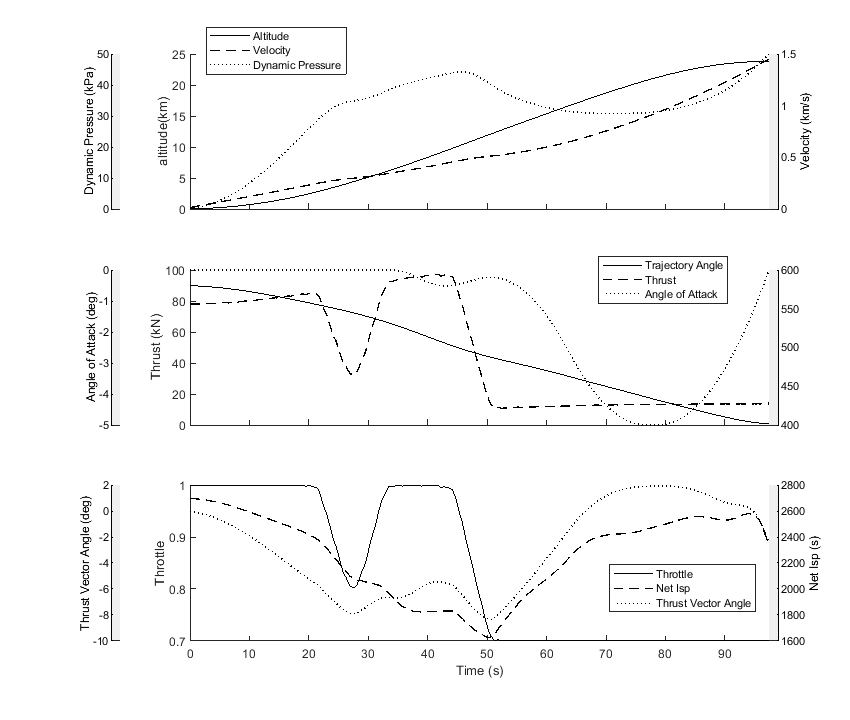
\includegraphics[width=0.9\linewidth]{H:/github-home/LODESTAR-revisions/ArchivedResults/20190809T122214mode900/FirstStageConstq}
	\caption{The first stage trajectory of the launch system, with the scramjet accelerator constrained to flight at constant dynamic pressure (Case 1).}
	\label{fig:FirstStageConstq}
\end{figure}
LODESTAR successfully computes the trajectory of the rocket-scramjet-rocket system, with the scramjet accelerator flying at constant dynamic pressure, achieving a payload-to-orbit of \PayloadToOrbitConstqNoReturn kg.
Figure \ref{fig:GroundTrackConstq} shows the optimised trajectory path, Figures \ref{fig:FirstStageConstq}-\ref{fig:ThirdStageConstq} show details of the optimised trajectory for each stage, and Table \ref{tab:constqsummary} provides a summary of the key parameters of the trajectory, including the exergy efficiency of each stage.
The rocket-scramjet-rocket system launches vertically, flying a fixed vertical trajectory for 3.9s, after which a pitchover is initiated. Under power of the first stage rocket, the launch system begins pitching, flying north-west, over the Arafura Sea. 
After pitchover the angle of attack stays constant at 0$^\circ$ for \textcolor{red}{99.9}s, as shown in Figure \ref{fig:FirstStageConstq}. At this point, the angle of attack is reduced, reaching a minimum of \textcolor{red}{-5.0}$^\circ$, before increasing back up to 0$^\circ$ for stage separation. 
The scramjet accelerator is separated at a trajectory angle of \firstsecondSeparationgammaConstqNoReturn$^\circ$ at an altitude of \firstsecondSeparationAltConstqNoReturn km, at a flight time of \textcolor{red}{97.4}s, with a total ground distance of \FirstStageDistStandardNoReturn km covered under power of the first stage rocket. 
 In order to reach optimal first-second stage separation conditions, the first stage must launch with a lower-than-maximum fuel mass, to allow it to pitch in the correct manner. To achieve an optimal constant dynamic pressure trajectory, the first stage launches with a fuel mass of 17010kg, significantly lower than the full amount of allowable fuel mass, 17934kg. 
 \textcolor{red}{XXX change this}
The first stage rocket achieves an exergy efficiency of \firstExergyEffConstqNoReturn\%$\eta$ when separating the scramjet accelerator onto a constant dynamic pressure trajectory. 


\begin{figure}[ht!]% updated 14/8/19
\centering
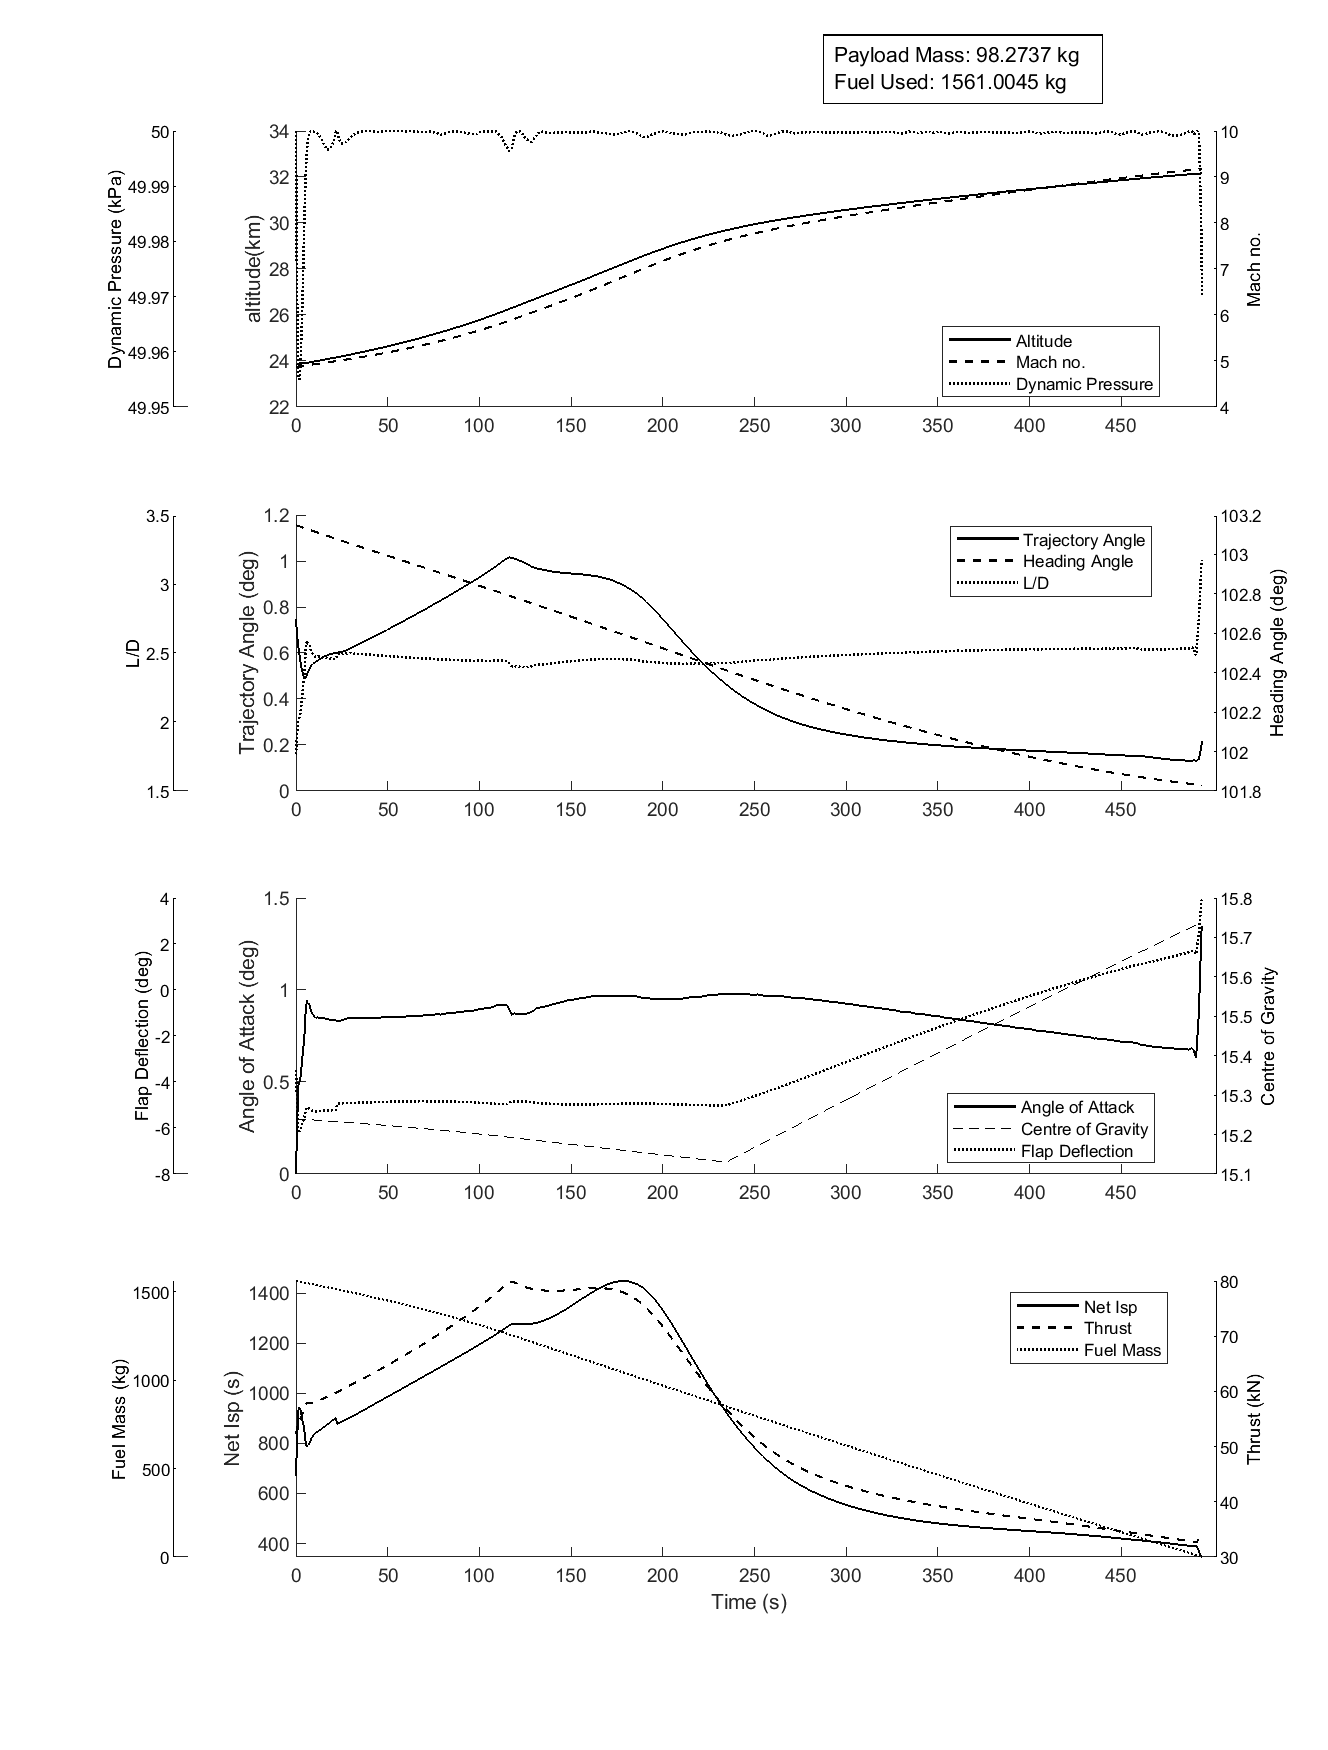
\includegraphics[width=0.9\linewidth]{H:/github-home/LODESTAR-revisions/ArchivedResults/20190809T122214mode900/SecondStageConstq}
\caption{The constant dynamic pressure flight path of the scramjet accelerator (Case 1).}
\label{fig:SecondStageConstq}
\end{figure}


The constant dynamic pressure trajectory for the scramjet accelerator stage is shown in Figure \ref{fig:SecondStageConstq}, with key results summarised in Table \ref{tab:constqsummary}. After the separation of the first stage rocket, the SPARTAN flies north west over the Arafura Sea, and crosses West Papua before releasing the third stage rocket. Due to the clear objective of a constant dynamic pressure trajectory, any deviations from the target dynamic pressure are readily apparent, allowing the efficacy of the optimiser to be verified. 
The constant dynamic pressure trajectory shows very close adherence to 50kPa dynamic pressure  throughout the trajectory (maximum 0.2\% deviation), indicating that scramjet accelerator flight at a constant dynamic pressure is able to be achieved by the SPARTAN.  
Over the trajectory, the Mach number increases from \textcolor{red}{4.88} to \textcolor{red}{9.18}, the velocity increases from \firstsecondSeparationvConstqNoReturn m/s to \secondthirdSeparationvConstqNoReturn m/s, and the flap deflection increases from \textcolor{red}{-6.14}$^\circ$ to \textcolor{red}{a maximum of 3.93$^\circ$ during pull-up}. The angles of attack of the scramjet accelerator are low across the trajectory, generally between \textcolor{red}{0.6-1.0}$^\circ$, indicating that the lift of the scramjet accelerator is high for this mission profile. At the beginning of the trajectory the equivalence ratio increases, as the capture limitations are relaxed with increasing Mach number. This causes the net specific impulse ($I_{sp_{net}} = \frac{T-D}{\dot{m}_f g}$) to increase, to a maximum of \textcolor{red}{1448s}, during the first \textcolor{red}{180.4}s flight time.  After this initial increase, the net specific impulse decreases over the trajectory, as the efficiency of the scramjet engines decreases. 
Third stage release occurs at\textcolor{red}{591.4s flight time}, at \secondthirdSeparationAltConstqNoReturn km altitude. Immediately before third stage separation, there is a slight increase in the angle of attack and flap deflection of the scramjet accelerator. This is done to increase the trajectory angle and improve the payload-to-orbit slightly, but does not have a significant effect on the performance of the launch system. 

\begin{figure}[ht!]% updated 14/8/19
\centering
\includegraphics[width=0.9\linewidth]{H:/github-home/LODESTAR-revisions/ArchivedResults/20190809T122214mode900/ThirdStageConstq}
\caption{The third stage trajectory of the launch system, with the scramjet accelerator constrained to flight at constant dynamic pressure (Case 1).}
\label{fig:ThirdStageConstq}
\end{figure}

Figure \ref{fig:ThirdStageConstq} shows the corresponding third stage atmospheric exit trajectory after release, evaluated as described in Chapter \ref{chapter:LODESTAR}. The third stage released from a constant dynamic pressure trajectory, shown in Figure \ref{fig:ThirdStageConstq}, is limited by the maximum thrust vector angle for the first 37.3s of flight. \textcolor{red}{XXX change this} This places significant limitations on the maximum allowable angle of attack. This angle of attack limitation reduces the lift of the rocket, causing the flight path angle to stay close to horizontal for the first \textcolor{red}{12}s of flight. This slow ascent leads to the rocket spending a large amount of time at low altitude, in a high drag environment, spending \thirdqOverFiveConstqNoReturn s at over 5kPa dynamic pressure. The angle of attack increases gradually to a maximum of \textcolor{red}{10}$^\circ$ at \textcolor{red}{27.8}s before decreasing until burnout at 130.4s\textcolor{red}{XXX change this}. The dynamic pressure of the third stage rocket reduces to 10kPa at \textcolor{red}{188.2}s, at which point the heat shield is discarded. The rocket coasts to a trajectory angle of 0$^\circ$, which is reached at a total flight time of \textcolor{red}{827.6}s. The trajectory terminates at 90km, the lowest allowable altitude for circularisation. 
When this altitude is reached, the trajectory is circularised and a Hohmann transfer manoeuvre is performed to reach sun synchronous orbit.






\section{Case 2: Optimised Ascent Trajectory}\label{sec:optimisednoreturn}

\textcolor{red}{XXX If i havent already, I should point out that the small corrections being made during 50kPa flight probably indicate that the vehicle shape is not optimised for 50kPa flight, and that it wants to fly at max q but cant sustain an optimal aoa to do so, link to prior work that showed similar?}

\textcolor{red}{XXX why is thrust vector angle so much larger here than for optimised ascent? is moment that much larger? I should note this if I havent already, that optimised stage will be much more controllable}

This section presents the maximum payload-to-orbit trajectory for the rocket-scramjet-rocket launch system, with the scramjet accelerator able to deviate from its maximum dynamic pressure. 
The optimal trajectory shape for a 50kPa dynamic pressure limited trajectory is shown in Figure \ref{fig:GroundTrackStandardNoReturn}, with detailed trajectory information for each stage shown in Figures \ref{fig:FirstStageStandardNoReturn} - \ref{fig:ThirdStageStandardNoReturn}, and key results summarised in Table \ref{tab:summaryStandardNoReturn}. The maximum payload-to-orbit trajectory shape involves the scramjet accelerator performing altitude raising manoeuvres, where the dynamic pressure of the scramjet accelerator is lowered from its maximum of 50kPa. These manoeuvres serve either to increase the net specific impulse of the scramjet accelerator, or to trade-off the efficiency of the scramjet accelerator in order to increase the efficiency of the first and third stages. 
This payload-to-orbit optimised trajectory is able to deliver \PayloadToOrbitStandardNoReturn kg of payload to heliocentric orbit, an increase of \textcolor{red}{59.1}\% over the constant, 50kPa dynamic pressure result (Case 1).

\begin{figure}[ht!]%updated 15/8/19
	
	
	
	\centering
	\includegraphics[width=1\linewidth]{H:/github-home/LODESTAR-revisions/ArchivedResults/20190723T125843mode10/GroundTrackStandard}
	\caption{The optimised maximum payload-to-orbit trajectory of the launch system (Case 2).}
	\label{fig:GroundTrackStandardNoReturn}
\end{figure}


The first stage, shown in Figure \ref{fig:FirstStageStandardNoReturn}, follows a very similar trajectory to that of the first stage releasing the scramjet accelerator onto a constant dynamic pressure trajectory.
\begin{figure}[ht!]% updated 14/8/19
	\centering
	\includegraphics[width=0.9\linewidth]{H:/github-home/LODESTAR-revisions/ArchivedResults/20190723T125843mode10/FirstStageStandard}
	\caption{The optimised maximum payload-to-orbit trajectory of the launch system under power of the first stage rocket (Case 2).}
	\label{fig:FirstStageStandardNoReturn}
\end{figure}
 However, the trajectory angle at the separation of the scramjet accelerator is \secondthirdSeparationgammaqStandardNoReturn$^\circ$, rather than the trajectory angle of \secondthirdSeparationgammaConstqNoReturn$^\circ$ required for the scramjet accelerator to fly a constant dynamic pressure trajectory. Additionally, the altitude at first-second stage separation is raised to \firstsecondSeparationAltStandardNoReturn km, an increase of \textcolor{red}{0.68}km compared to the separation point of a scramjet accelerator flying at constant 50kPa dynamic pressure. This higher release angle and altitude causes the altitude of the scramjet accelerator to initially increase, and consequently for its dynamic pressure to decrease. This increased trajectory angle at separation is the consequence of a trade-off between the efficiency of the scramjet accelerator, and the efficiency and fuel mass of the first stage. 
 In order to release the scramjet accelerator at a trajectory angle conducive to flying at a constant 50kPa dynamic pressure, the first stage must launch with a low fuel mass, to allow it to pitch in the correct manner. When the scramjet accelerator release angle and altitude are able to increase, the first stage is launched with a fuel mass of 17185kg, an increase of 1.0\% compared to the constant dynamic pressure trajectory in Case 1.\textcolor{red}{XXX change this} This additional fuel and efficiency result in more energy being imparted upon the scramjet accelerator, \firstdExergyStandardNoReturn GJ, compared to \firstdExergyConstqNoReturn GJ when being released onto a 50kPa trajectory. 
 In addition, the efficiency of the first stage is increased to \firstExergyEffStandardNoReturn\%$\eta$ due to the increased acceleration, an overall improvement of +0.148\%$\eta$ (+2.4\%) compared to the first stage separating the scramjet accelerator at 50kPa conditions. \textcolor{red}{XXX update this}
 During the maximum payload-to-orbit trajectory, the first stage rocket releases the scramjet accelerator at a velocity of \firstsecondSeparationvStandardNoReturn m/s, an increase of \textcolor{red}{5.7}\% compared to the first stage releasing the scramjet accelerator onto a constant dynamic pressure trajectory. Neither first stage utilises the full amount of allowable fuel mass, 17934kg, indicating that using the full fuel mass would necessitate separation conditions which would reduce the efficiency of the scramjet accelerator unfavourably. \textcolor{red}{XXX change this}
These results indicate that the fuel mass utilised by the first stage has an optimal magnitude, and that including additional fuel past this amount does not increase the performance of the system. This implies that the size of the first stage is closely linked to the optimal trajectory of the system, and that future first stage designs should be sized so that optimal pitching is achieved. 

\begin{table}[ht]% updated 14/8/19
	\centering
\begin{tabular}{l c } 
	\hline \textbf{Trajectory Condition}
	& Value
	\\
	\hline \textbf{Payload to Orbit (kg)}
	& \textbf{\PayloadToOrbitStandardNoReturn}
	\\
	\textbf{Total $\eta_{exergy}$ (\%)}
	& \textbf{\totalExergyEffStandardNoReturn}
	\\
	\hline 
	\textbf{1$^{st}$ Stage $\eta_{exergy}$ (\%)}
	& \textbf{\firstExergyEffStandardNoReturn}
	\\

	\textbf{Separation Alt, 1$\rightarrow$2 (km)}
	& \firstsecondSeparationAltStandardNoReturn
	\\
	\textbf{Separation v, 1$\rightarrow$2 (m/s)}
	& \firstsecondSeparationvStandardNoReturn
	\\
	\textbf{Separation $\gamma$, 1$\rightarrow$2 (deg)}
	& \firstsecondSeparationgammaStandardNoReturn
	\\
	\hline 
	\textbf{2$^{nd}$ Stage $\eta_{exergy}$ (\%)}
	& \textbf{\secondExergyEffStandardNoReturn}
	\\

	\textbf{Separation Alt, 2$\rightarrow$3 (km)}
	& \secondthirdSeparationAltStandardNoReturn
	\\
	\textbf{Separation $v$, 2$\rightarrow$3 (m/s)}
	& \secondthirdSeparationvStandardNoReturn
	\\
	\textbf{Separation $\gamma$, 2$\rightarrow$3 (deg)}
	& \secondthirdSeparationgammaStandardNoReturn
	\\
	\textbf{2$^{nd}$ Stage Distance Flown (km)}
	& \SecondDistStandardNoReturn
	\\
	\hline 
	\textbf{3$^{rd}$ Stage $\eta_{exergy}$ (\%)}
	& \textbf{\thirddExergyEffStandardNoReturn}
	\\

	\textbf{3$^{rd}$ Stage $t$, $q >$ 5kpa (s)}
	& \thirdqOverFiveStandardNoReturn
	\\
	\textbf{3$^{rd}$ Stage max $\alpha$ (deg)}
	& \thirdmaxAoAStandardNoReturn
	\\
	\textbf{3$^{rd}$ Stage Fuel Mass (kg)}
	& \thirdmFuelStandardNoReturn
	\\
	\hline 
\end{tabular} 
	\caption{A summary of key results from the maximum payload-to-orbit trajectory (Case 2).}
	\label{tab:summaryStandardNoReturn}
\end{table}







\begin{figure}[ht!]% updated 14/8/19
\centering
\includegraphics[width=0.9\linewidth]{H:/github-home/LODESTAR-revisions/ArchivedResults/20190723T125843mode10/SecondStageStandard}
\caption{The optimised maximum payload-to-orbit trajectory of the scramjet accelerator (Case 2).}
\label{fig:SecondStageStandardNoReturn}
\end{figure}



After the initial deviation from the maximum dynamic pressure, the scramjet accelerator returns to 50kPa dynamic pressure for a time. 
At \textcolor{red}{184.9} seconds flight time, the altitude of the trajectory is again raised, and the dynamic pressure decreased, to a minimum of \textcolor{red}{43.0}kPa. In this region the net specific impulse of the scramjet accelerator is relatively homogeneous with respect to changes in dynamic pressure, as can be observed in the specific impulse of the C-REST engines in Figure \ref{fig:IspStandard}. The homogeneity between flight conditions means that the variation in engine performance with flight conditions is small and that flying at the maximum dynamic pressure in this region does not maximise the specific impulse from the C-REST engines. Figure \ref{fig:NetIspStandardNoReturn} shows that while the optimised trajectory differs significantly from a constant dynamic pressure trajectory, both achieve similar net specific impulses during the acceleration phase of flight, with the exception of the initial trajectory conditions at Mach 5, where the efficiency of the scramjet accelerator is traded for first stage rocket performance. 
Appendix \ref{sec:Appendix_qconst} details a maximum payload-to-orbit trajectory in which the scramjet accelerator is constrained to 50kPa between Mach 6-8, to prevent the altitude raising manoeuvre from taking place. This constrained trajectory allows for the magnitude of the performance gain from the altitude raising manoeuvre to be quantified. 
Overall, the altitude raising manoeuvre results in a slight increase in net specific impulse, compared to the trajectory constrained to maximum $q$, increasing the overall efficiency of the launch system from \totalExergyEffqconstrainedNoReturn \%$\eta$ to \totalExergyEffStandardNoReturn\%$\eta$. This is a relatively minor variation, and the payload-to-orbit benefits of this altitude raising manoeuvre are correspondingly small; 
the optimised trajectory exhibits a payload-to-orbit increase of 0.4kg compared to the trajectory constrained to 50kPa between Mach 6-8, a difference of only 0.2\%. \textcolor{red}{XXX update this with new constrained traj}
However, it is important to note that, while its benefits are small, the altitude raising manoeuvre is consistently observed in all maximum payload-to-orbit optimised trajectories in which dynamic pressure is unconstrained. 
Also, despite its small benefit to payload-to-orbit, this altitude raising manoeuvre is significant as it reduces the heating and structural loading on the scramjet accelerator, though it is beyond the scope of this study to quantify these benefits. 
\textcolor{red}{XXX link to other studies that showed off max q flight}



\begin{figure}[ht!]% updated 14/8/19 - note, modified point location for Mach 8.5 so not to be during pull-up
	\centering
	\includegraphics[width=\linewidth]{H:/github-home/LODESTAR-revisions/ArchivedResults/20190723T125843mode10/NetIspStandard}
	\caption{Net Isp contours for the scramjet accelerator at Mach numbers from 5-9, showing flight conditions for an optimised trajectory with no constraints (Case 2) and a constant dynamic pressure trajectory (Case 1). }
	\label{fig:NetIspStandardNoReturn}
\end{figure}

\begin{figure}[ht!]% updated 14/8/19 
	\centering
	\includegraphics[width=0.8\linewidth]{H:/github-home/LODESTAR-revisions/ArchivedResults/20190723T125843mode10/IspStandard}
	\caption{The specific impulse of the C-REST engines, plotted for inlet temperature (T1) and inlet Mach number (M1). Data points are shown in black.}
	\label{fig:IspStandard}
\end{figure}


At \textcolor{red}{319.4}s, the scramjet accelerator returns to flight at close to 50kPa dynamic pressure until \textcolor{red}{511.1}s, at which point a pull-up manoeuvre is performed, gaining altitude until the third stage rocket is released at \textcolor{red}{543.7}s of scramjet accelerator flight time. 
 The point at which the pull-up manoeuvre begins is the location that takes into account the best combination of velocity, altitude and release angle for the trade-off between the scramjet stage performance and the release of the third stage rocket. This pull-up indicates the region at which increasing altitude and release angle becomes more important than extracting maximum thrust from the scramjet (which is generally attained at high $q$ and low flight angle at an equivalence ratio of 1).
At high Mach numbers, flight in a lower dynamic pressure environment results in less thrust output from the scramjet engines, as well as an increase in angle of attack and flap deflection angle to compensate for the additional lift required. Due to this, less overall acceleration is obtained compared to the fixed dynamic pressure result. Separation occurs at a velocity of \secondthirdSeparationvStandardNoReturn m/s, a decrease of \textcolor{red}{145.0}m/s (\textcolor{red}{-5.2}\%). However, at the same time separation altitude increases by \textcolor{red}{11.65}km (+\textcolor{red}{36.2}\%) to \secondthirdSeparationAltqStandardNoReturn km, resulting in a decrease in separation dynamic pressure to \secondthirdSeparationqStandardNoReturn kPa. 
\begin{figure}[ht!]% updated 14/8/19
	\centering
	\includegraphics[width=0.9\linewidth]{H:/github-home/LODESTAR-revisions/ArchivedResults/20190723T125843mode10/ThirdStageStandard}
	\caption{The third stage trajectory of the launch system flying the maximum payload-to-orbit trajectory (Case 2).}
	\label{fig:ThirdStageStandardNoReturn}
\end{figure}
The scramjet stage pull-up assists the rocket in manoeuvring to exoatmospheric altitude by increasing the altitude and angle at separation, utilising the superior aerodynamics and manoeuvrability of the scramjet accelerator. The increase in release angle, to the optimal angle of \secondthirdSeparationgammaStandardNoReturn$^\circ$, significantly reduces the turning that is required by the rocket as evident from comparing Fig \ref{fig:ThirdStageConstq} and \ref{fig:ThirdStageStandardNoReturn}. 
Overall, the altitude raising manoeuvres which the scramjet accelerator performs result in a decrease in the exergy efficiency of the scramjet accelerator to \secondExergyEffStandardNoReturn\%$\eta$, a total decrease of \textcolor{red}{-0.719}\%$\eta$ (-\textcolor{red}{14.04}\%) compared to the scramjet accelerator flying at a constant dynamic pressure. However, the optimised trajectory drastically increases the exergy efficiency of the third stage, to \thirddExergyEffStandardNoReturn\%$\eta$, an overall increase of +\textcolor{red}{6.013}\%$\eta$ (\textcolor{red}{+63.20}\%) compared to the third stage released from the scramjet accelerator flying a fixed dynamic pressure trajectory.  
Along with the increased efficiency of the first stage, this exergy trade-off leads to the total exergy efficiency of the launch system increasing, from \totalExergyEffConstqNoReturn\%$\eta$ to \totalExergyEffStandardNoReturn\%$\eta$. 

The trajectory of the third stage rocket after release from an optimised scramjet trajectory is shown in Figure \ref{fig:ThirdStageStandardNoReturn}. Release at a higher, more optimal angle, reduces the aerodynamic moment necessary to trim the vehicle. In turn, this reduced moment reduces the necessary thrust vector angle, so that the thrust vector limit is not reached. The third stage rocket is released at a high trajectory angle, and continuously gains altitude, avoiding the close-to-horizontal flight required by the fixed dynamic pressure release (Case 1).
Due to the higher altitude and release angle, the third stage rocket is released at a lower dynamic pressure, \secondthirdSeparationqCdStandardNoReturn kPa compared to \secondthirdSeparationqConstqNoReturn kPa, and spends much less time flying in a high dynamic pressure environment, \thirdqOverFiveStandard s at over 5kPa dynamic pressure rather than \thirdqOverFiveConstqNoReturn s. 
The reduced time that the rocket must spend in a high dynamic pressure environment, and the decrease in the maximum dynamic pressure that the rocket stage experiences, may allow the structural mass and heat shielding necessary to achieve exoatmospheric flight to be decreased. This reduced mass may enable higher payload to orbit, though it is beyond the scope of this study to investigate these design changes. \textcolor{red}{XXX link to section where I do this}

\textcolor{red}{XXX update this para}
Previous studies considering the optimised trajectory of vehicles with multiple propulsion methods within a single stage show airbreathing-rocket transitions at, or close to, exoatmospheric flight, at altitudes from 56-130km\cite{Lu1993,Trefny1999,Bradford2000}. Compared to these studies, the maximum payload to orbit trajectory of the multi-stage system shows a scramjet-rocket transition point at much lower altitudes.
This lower transition point is a consequence of the stage separation creating an energy trade-off between the stages, which does not occur in a single stage vehicle. Single-stage vehicles must necessarily transport all components to exoatmosphere, and so utilise the scramjet engines until higher altitude to take advantage of their high efficiency. A multi-stage vehicle is able to separate the scramjet stage. 
This separation occurs when the performance benefits provided by the superior aerodynamics and engine efficiency of the scramjet stage are offset by the energy required to lift the extra mass to higher altitude. The beneficial ability
to separate the scramjet stage results in a lower altitude scramjet-rocket transition point, when compared to single
stage vehicle designs.



\section{Energy Usage Analysis}\label{sec:exergy1}


\begin{table}[ht] % updated 15/8/19, note, ive just rounded the numbers, even though they dont quite add up right, seems most logical
	\centering
	\begin{tabular}{l c c} 
		\hline \textbf{Trajectory Condition}
		&50kpa Constant $q$
		&No $q$ Constraint
		\\
		\textbf{First Stage Fuel Exergy} 
		&\textbf{\firstEnergyConstqNoReturn} GJ
		&\textbf{\firstEnergyStandardNoReturn} GJ
		\\
		
		\textcolor{blue}{KE + PE of Payload}
		& \firstWpayloadConstqNoReturn \% (0.13 GJ)
		& \firstWpayloadStandardNoReturn \% (0.22 GJ)
		\\
		\textcolor{red}{KE + PE of  2$^{nd}$ \& 3$^{rd}$ Stage}
		& \firstWnextStageConstqNoReturn \% (12.50 GJ) & \firstWnextStageStandardNoReturn \% (13.66 GJ)
		\\
		
		\textcolor{red}{Overcoming Drag} 
		& \WDoneConstqNoReturn \% (5.57 GJ) & \WDoneStandardNoReturn \% (5.03 GJ)
		\\
		\textcolor{red}{KE + PE of 1$^{st}$ Stage Structural Mass} 
		& \WoneConstqNoReturn \% (1.86 GJ) & \WoneStandardNoReturn \% (2.04 GJ)
		\\ 
		\textcolor{red}{Propulsion Inefficiency} 
		& \PlossoneCombinedConstqNoReturn (181.84 GJ) \% & \PlossoneCombinedStandardNoReturn \% (180.95 GJ)
		\\ 
		\textbf{scramjet accelerator Fuel Exergy} 
		& \textbf{\secondEnergyConstqNoReturn} GJ & \textbf{\secondEnergyStandardNoReturn} GJ
		\\
		\textcolor{blue}{KE + PE of Payload}
		& \secondWpayloadConstqNoReturn \% (0.28 GJ) & \secondWpayloadStandardNoReturn \% (0.39 GJ) 
		\\
		\textcolor{red}{KE + PE of 3$^{rd}$ Stage}
		& \secondWnextStageConstqNoReturn \% (9.31 GJ) & \secondWnextStageStandardNoReturn \% (7.85 GJ)
		\\
		\textcolor{red}{Overcoming Drag}
		& \WDsecondConstqNoReturn \% (35.00 GJ) & \WDsecondStandardNoReturn \% (38.26 GJ)
		\\
		\textcolor{red}{KE + PE of scramjet accelerator Structural Mass}  
		& \WsecondConstqNoReturn \% (14.40 GJ) & \WsecondStandardNoReturn \% (12.39 GJ)
		\\
		\textcolor{red}{Propulsion Inefficiency}  
		& \PlosssecondCombinedConstqNoReturn \% (128.37 GJ) & \PlosssecondCombinedStandardNoReturn \% (128.49 GJ)
		\\
		
		\textbf{Third Stage Fuel Exergy}  
		& \textbf{\thirdEnergyConstqNoReturn}  GJ & \textbf{\thirdEnergyStandardNoReturn}  GJ
		\\
		\textcolor{blue}{KE + PE of Payload}  
		&\thirddExergyEffConstqNoReturn \% (3.33 GJ) &\thirddExergyEffStandardNoReturn \% (5.33 GJ)
		\\
		\textcolor{red}{Overcoming Drag}  
		& \WDthreeConstqNoReturn \% (2.98 GJ) & \WDthreeStandardNoReturn \% (0.11 GJ)
		\\
		\textcolor{red}{KE + PE  of 3$^{rd}$ Stage Structural Mass}  
		& \WthreeConstqNoReturn \% (10.49 GJ) & \WthreeStandardNoReturn \% (10.59 GJ)
		\\
		
		\textcolor{red}{KE + PE of Heat Shield}  
		
		& \WHSthreeConstqNoReturn \% (2.96 GJ) & \WHSthreeStandardNoReturn \% (1.22 GJ)
		\\
		
		\textcolor{red}{Propulsion Inefficiency}  
		& \PlossthreeCombinedConstqNoReturn \% (15.25 GJ) & \PlossthreeCombinedStandardNoReturn \% (17.07 GJ)
		\\
		\hline 
	\end{tabular} 
	\caption{An energy usage breakdown of the ascent trajectories, both with, and without, the scramjet accelerator constrained to constant dynamic pressure (Cases 1 \& 2). Blue indicates a 'productive' energy usage, whereas red indicates energy 'wastage'. \textcolor{red}{XXX fix all to be same s.f.}}
	\label{tab:effStandardNoReturn}
\end{table}



An energy usage analysis is conducted on the maximum payload-to-orbit launch trajectories, both with, and without the scramjet accelerator constrained to constant dynamic pressure flight (Cases 1 \& 2). This is performed in order to understand the primary sources of energy loss for each stage, and to compare the trajectories optimised with, and without the scramjet accelerator constrained to constant dynamic pressure. An energy usage breakdown of each of each stage is compared in Table \ref{tab:effStandardNoReturn}. The energy usage breakdown compares: the energy used to accelerate the payload, $\Delta KE_{payload} + \Delta PE_{payload}$; the energy imparted to the successive stages, $\Delta KE_{next stage} + \Delta PE_{next stage}$; the energy used overcoming drag, $\int_{t_0}^{t_f} v\,D \, dt$; the energy used imparting energy to the structural mass of each stage, which is separated, $\Delta KE_{discarded} + \Delta PE_{discarded}$; and the energy lost due to propulsion inefficiency. 



 The efficiency of the first stage rocket increases when the first-second stage separation altitude and trajectory angle are raised, in the trajectory with no dynamic pressure constraint. 
 This is due to the lower propulsive efficiency of rockets at low speeds, illustrated by the equation for the propulsive efficiency of a rocket\cite{RPE}:
 \begin{equation}\label{eq:rocketeff}
 \eta_P = \frac{2\,v_0/v_g}{1\,+\,(v_0/v_g)^2}, 
 \end{equation}
 where $v_g$ is the exhaust velocity, and $v_0$ is the velocity of the vehicle.
 At low rocket velocities there is a large difference between the flight speed of the vehicle, and the exhaust velocity of the rocket engine, resulting in low propulsion efficiencies, and consequently high propulsive inefficiency losses. 
 The propulsive losses of the first stage rocket decrease when the scramjet accelerator is not constrained to a constant dynamic pressure trajectory, as a consequence of the additional acceleration obtained from the larger fuel exergy. 
 However, due to the first stage rocket starting from rest, the first stage rocket always loses a large portion of its exergy to propulsion inefficiency.  
 
The energy imparted upon the payload and third stage rocket during the scramjet accelerator's acceleration is decreased significantly when the scramjet accelerator is allowed to deviate from 50kPa dynamic pressure, reducing from \textcolor{red}{9.31}GJ to \textcolor{red}{7.85}GJ, a decrease of \textcolor{red}{-15.7}\%. This energy is traded-off during the pull-up manoeuvre, by utilising the superior aerodynamics of the scramjet accelerator to manoeuvre into flight conditions that are favourable for the separation of the third stage, improving the efficiency of the third stage ascent. Even though less energy is imparted upon the third stage before separation, a release from the end of a scramjet accelerator pull-up enables the third stage to impart significantly more energy onto the payload, at \textcolor{red}{5.33}GJ, compared to \textcolor{red}{3.33}GJ when released from 50kPa, an increase of \textcolor{red}{+60.1}\%, with a significantly increased exergy efficiency of \thirddExergyEffStandardNoReturn \%.  

The additional energy efficiency of the third stage comes from a decrease in the energy lost due to drag, as well as a decrease in the energy imparted upon the heat shield. 
The energy lost from the third stage overcoming drag is dependent on the amount of time that the rocket spends in the atmosphere, and comprises \WDthreeConstqNoReturn \% of the fuel exergy when released at 50kPa, and \WDthreeStandardNoReturn \% when released after a pull-up of the scramjet accelerator.
The energy lost accelerating the heat shield is also significantly larger when released from the scramjet accelerator flying a constant dynamic pressure trajectory, at \WHSthreeConstqNoReturn \% of the fuel exergy, compared to only \WHSthreeStandardNoReturn \% when the third stage is released after a pull-up of the scramjet accelerator. This is due to the third stage spending considerably more time in a high dynamic pressure environment when released from a constant dynamic pressure trajectory, requiring the heat shield for longer, so that more kinetic and potential energy is imparted upon the heat shield during acceleration. However, the energy losses due to the propulsion inefficiency of the third stage are higher when released from the end of a scramjet accelerator pull-up, compared to the trajectory constrained to constant dynamic pressure. This is due to the third stage being released at lower velocity, from the end of a scramjet accelerator pull-up manoeuvre, resulting in a lower efficiency as illustrated in Equation \ref{eq:rocketeff}. This indicates that there is a trade-off between the propulsion inefficiencies of the third stage, and the drag and heat shield energy losses.


The propulsion inefficiency losses of the scramjet accelerator are relatively low, compared to those of the first stage.
These lowered propulsion losses are due to the scramjet accelerator's engines utilising atmospheric oxygen as an oxidiser, resulting in a higher propulsion system efficiency.
%\cite{Spittle2003}:
%\begin{equation}
%\eta_P = \frac{2}{1\,+\,v_g/v_0}. 
%\end{equation}
 However, the scramjet accelerator loses a large amount of its exergy to overcoming drag. These high drag losses are due to the scramjet accelerator accelerating at high speeds within the atmosphere, at high dynamic pressures, and serve to partially offset the reduced energy losses due to the high propulsive efficiency of the scramjet accelerator. 
 The drag losses of the scramjet accelerator flying a trajectory with no dynamic pressure constraint are higher than those of the scramjet accelerator flying a constant dynamic pressure trajectory, at \WDsecondStandardNoReturn\%, compared to \WDsecondConstqNoReturn\%. This is due to the additional manoeuvring of the scramjet accelerator during the pull-up before third stage release when the dynamic pressure is not constrained, which requires high angles of attack, and increases drag significantly. 
 
 The propulsive energy losses of the third stage are also low, compared to the first stage rocket. This is due to the larger velocity of the third stage, compared to the first stage, which increases the propulsive efficiency of the third stage rocket.
 


 

  

\section{Sensitivity Analysis}\label{sec:sensitivityNoReturn}
\textcolor{red}{XXX add first stage thrust and mass variation? ... maybe if i think its worth it}

\textcolor{red}{XXX I need more justification and estimation of variance (can maybe look at dawids and other shape optimisation papers to get an idea?) I also need to focus this partly in terms of uncertainties}

\textcolor{red}{XXX I need to make it clear that the sensitivity study is an important contribution, that gives useful insights into the interplay between the stages}

\textcolor{red}{XXX I need to make clear that this analysis isnt just 'what are the number differences' but mostly 'is the trajectory optimisation valid across vehicle designs'}


\textcolor{red}{XXX remove max aoa form tables}

\textcolor{red}{The launch system studied in this work is intended to be representative of a three stage, rocket-scramjet-rocket, small satellite launch system, to be used to inform future vehicle designs. It is anticipated that the design of the launch system will change significantly before a optimal, or even practically feasible, iteration is reached. Additionally, this study models the launch system using medium and low fidelity methods, which may be significant sources of error on the final optimised trajectory.  
	To quantify how variations in a the design of a stage or variations in the performance of a stage due to modelling error may affect the performance of the launch system, it is useful to conduct a sensitivity analysis on the launch system.}
A sensitivity analysis is conducted, in which selected design parameters of the launch system are varied, and the effects on the optimised maximum payload-to-orbit trajectory of the launch system are investigated. Appendix \ref{sec:Appendix_trajectorycomparisons} shows comparison plots of the scramjet accelerator and third stage trajectories for each parameter variation study, however, the first stage rocket trajectories are very similar and are not compared graphically. Key results including performance factors of each stage and separation conditions are summarised within this section.
This study is performed in order to determine the relative importance of the design parameters on the efficiency of the system, as well as investigating changes in the maximum payload-to-orbit trajectory as the performance of the launch system is varied. The investigation of the key design parameters of the launch system provides a comparative metric, which is used to quantify the relative impact of the vehicle design on the performance of the launch system. The performance trade-offs between the stages are investigated by studying the variation in the optimised trajectory, particularly the stage separation conditions, as the parameters of the launch system design are changed. 
Trends are developed for each parameter study, quantifying how much the performance factors of the launch system vary per percentage of variation of each design parameter ($\Delta$/$\Delta$\%). This percentage variation gives a general metric for how much each design parameter effects the performance factors of the launch system. However, the relative magnitude of one percent variation of each individual design parameter must be taken into account when making comparisons. 

The information obtained from this parameter variation study can be used to inform future launch system designs. 
In addition, this sensitivity study serves to verify the ability of LODESTAR to generate optimal trajectories with varied vehicle designs, as well as investigating the robustness of the optimised solution with respect to uncertainties in the vehicle design and performance.
When necessary for the trajectory simulations within this section, it is assumed that the scramjet engines are operable at velocities slightly under Mach 5. This assumption is made in order to allow meaningful assessment of parameters which effect the first-second stage separation velocity, without modification of the first stage rocket.
All optimised trajectories within this section use the full amount of fuel available to the scramjet accelerator vehicle. 


\subsection{Case 3: Maximum Dynamic Pressure Sensitivity}\label{sec:qvariation}


\begin{table}[ht!]
	\centering
	\begin{tabular}{l c c c c c c} 
		\hline \textbf{Trajectory Condition  \qquad  $q_{max}$: }
		&40kPa
		&45kPa
		&50kPa
		& 55kPa
		& 60kPa
		& $\Delta/\Delta$\%q
	\\
	\hline \textbf{Payload to Orbit (kg)}
	& \textbf{\PayloadToOrbitqFortyNoReturn}
	& \textbf{\PayloadToOrbitqFortyFiveNoReturn}
	& \textbf{\PayloadToOrbitqStandardNoReturn}
	& \textbf{\PayloadToOrbitqFiftyFiveNoReturn}
	& \textbf{\PayloadToOrbitqSixtyNoReturn}
	&\textbf{0.4}
	\\
	\textbf{Payload Variation (\%)}
	& \PayloadVarqFortyNoReturn
	& \PayloadVarqFortyFiveNoReturn
	& \PayloadVarqStandardNoReturn
	& \PayloadVarqFiftyFiveNoReturn
	& \PayloadVarqSixtyNoReturn
	&0.2
	\\
	\textbf{Total $\eta_{exergy}$ (\%)}
	& \textbf{\totalExergyEffqFortyNoReturn}
	& \textbf{\totalExergyEffqFortyFiveNoReturn}
	& \textbf{\totalExergyEffqStandardNoReturn}
	& \textbf{\totalExergyEffqFiftyFiveNoReturn}
	& \textbf{\totalExergyEffqSixtyNoReturn}
	& \textbf{3e-05}
	\\
	\hline 
	\textbf{1$^{st}$ Stage $\eta_{exergy}$ (\%)}
	& \textbf{\firstExergyEffqFortyNoReturn}
	& \textbf{\firstExergyEffqFortyFiveNoReturn}
	& \textbf{\firstExergyEffqStandardNoReturn}
	& \textbf{\firstExergyEffqFiftyFiveNoReturn}
	& \textbf{\firstExergyEffqSixtyNoReturn}
	& \textbf{-0.002}
	\\

	\textbf{Separation Alt, 1$\rightarrow$2 (km)}
	& \firstsecondSeparationAltqFortyNoReturn
	& \firstsecondSeparationAltqFortyFiveNoReturn
	& \firstsecondSeparationAltqStandardNoReturn
	& \firstsecondSeparationAltqFiftyFiveNoReturn
	& \firstsecondSeparationAltqSixtyNoReturn
	&-0.06
	\\
	\textbf{Separation v, 1$\rightarrow$2 (m/s)}
	& \firstsecondSeparationvqFortyNoReturn
	& \firstsecondSeparationvqFortyFiveNoReturn
	& \firstsecondSeparationvqStandardNoReturn
	& \firstsecondSeparationvqFiftyFiveNoReturn
	& \firstsecondSeparationvqSixtyNoReturn
	& -
	\\
	\textbf{Separation $\gamma$, 1$\rightarrow$2 (deg)}
	& \firstsecondSeparationgammaqFortyNoReturn
	& \firstsecondSeparationgammaqFortyFiveNoReturn
	& \firstsecondSeparationgammaqStandardNoReturn
	& \firstsecondSeparationgammaqFiftyFiveNoReturn
	& \firstsecondSeparationgammaqSixtyNoReturn
	&-0.13
	\\
	\hline 
	\textbf{2$^{nd}$ Stage $\eta_{exergy}$ (\%)}
	& \textbf{\secondExergyEffqFortyNoReturn}
	& \textbf{\secondExergyEffqFortyFiveNoReturn}
	& \textbf{\secondExergyEffqStandardNoReturn}
	& \textbf{\secondExergyEffqFiftyFiveNoReturn}
	& \textbf{\secondExergyEffqSixtyNoReturn}
	& \textbf{0.008}
	\\

	\textbf{Separation Alt, 2$\rightarrow$3 (km)}
	& \secondthirdSeparationAltqFortyNoReturn
	& \secondthirdSeparationAltqFortyFiveNoReturn
	& \secondthirdSeparationAltqStandardNoReturn
	& \secondthirdSeparationAltqFiftyFiveNoReturn
	& \secondthirdSeparationAltqSixtyNoReturn
	&-0.02
	\\
	\textbf{Separation $v$, 2$\rightarrow$3 (m/s)}
	& \secondthirdSeparationvqFortyNoReturn
	& \secondthirdSeparationvqFortyFiveNoReturn
	& \secondthirdSeparationvqStandardNoReturn
	& \secondthirdSeparationvqFiftyFiveNoReturn
	& \secondthirdSeparationvqSixtyNoReturn
	&1.56
	\\
	\textbf{Separation $\gamma$, 2$\rightarrow$3 (deg)}
	& \secondthirdSeparationgammaqFortyNoReturn
	& \secondthirdSeparationgammaqFortyFiveNoReturn
	& \secondthirdSeparationgammaqStandardNoReturn
	& \secondthirdSeparationgammaqFiftyFiveNoReturn
	& \secondthirdSeparationgammaqSixtyNoReturn
	&0.03
	\\
	\textbf{2$^{nd}$ Stage Distance Flown (km)}
	& \SecondDistqFortyNoReturn
	& \SecondDistqFortyFiveNoReturn
	& \SecondDistqStandardNoReturn
	& \SecondDistqFiftyFiveNoReturn
	& \SecondDistqSixtyNoReturn
	&-7.4
	\\
	\hline 
	\textbf{3$^{rd}$ Stage $\eta_{exergy}$ (\%)}
	& \textbf{\thirddExergyEffqFortyNoReturn}
	& \textbf{\thirddExergyEffqFortyFiveNoReturn}
	& \textbf{\thirddExergyEffqStandardNoReturn}
	& \textbf{\thirddExergyEffqFiftyFiveNoReturn}
	& \textbf{\thirddExergyEffqSixtyNoReturn}
	& \textbf{0.037}
	\\

	\textbf{3$^{rd}$ Stage $t$, $q >$ 5kpa (s)}
	& \thirdqOverFiveqFortyNoReturn
	& \thirdqOverFiveqFortyFiveNoReturn
	& \thirdqOverFiveqStandardNoReturn
	& \thirdqOverFiveqFiftyFiveNoReturn
	& \thirdqOverFiveqSixtyNoReturn
	& -
	\\
	\textbf{3$^{rd}$ Stage max $\alpha$ (deg)}
	& \thirdmaxAoAqFortyNoReturn
	& \thirdmaxAoAqFortyFiveNoReturn
	& \thirdmaxAoAqStandardNoReturn
	& \thirdmaxAoAqFiftyFiveNoReturn
	& \thirdmaxAoAqSixtyNoReturn
	&0
	\\
	\textbf{3$^{rd}$ Stage Fuel Mass (kg)}
	& \thirdmFuelqFortyNoReturn
	& \thirdmFuelqFortyFiveNoReturn
	& \thirdmFuelqStandardNoReturn
	& \thirdmFuelqFiftyFiveNoReturn
	& \thirdmFuelqSixtyNoReturn
	&-0.37
	\\
	\hline 
\end{tabular}  
	\caption{Comparison of key trajectory parameters with variation in the maximum dynamic pressure of the scramjet accelerator (Case 3).}
	\label{tab:qvarnoreturn}
\end{table}





To investigate the sensitivity of the vehicle to changes in $q_{max}$, the maximum permissible dynamic pressure is varied by $\pm$10kPa in 5kPa increments, and the flight trajectory optimised, with results shown in Table \ref{tab:qvarnoreturn}, and comparison plots shown in Appendix \ref{sec:app_comparison20}.
The variation in maximum dynamic pressure has only a small effect on the total exergy efficiency of the system, and hence only a small effect on the payload mass delivered to sun synchronous orbit.  Varying the maximum dynamic pressure by $\pm20\%$ causes a variation of only +0.064\%$\eta$ or -0.069\%$\eta$ in the exergy efficiency of the launch system and a corresponding +7.2kg (+3.82\%) or -7.8kg (-4.11\%) variation in the payload to orbit.  
The scramjet accelerator pull-up manoeuvres of all cases are similar, with a slight trend of decreasing altitude as the maximum dynamic pressure is increased. Altitudes of \secondthirdSeparationAltqFortyNoReturn km and \secondthirdSeparationAltqSixtyNoReturn km are reached for the 40kPa and 60kPa limited cases respectively, with separation velocities of \secondthirdSeparationvqFortyNoReturn m/s and \secondthirdSeparationvqSixtyNoReturn m/s. The 40kPa limited case flies for 612.1s, significantly longer than the 60kPa limited case, which flies for 468.1s.
As the dynamic pressure decreases, the size of the altitude raising manoeuvre in the middle of the trajectory decreases. This is due to the increased altitude and angle of attack moving the flight conditions into a region where the specific impulse of the C-REST engines is not homogeneous, so that it is beneficial to fly at maximum dynamic pressure.  
All trajectories pull-up to similar altitudes, with a relatively small variation in separation velocity of +33m/s (+1.2\%) and -30m/s (-1.1\%).
This small variation in velocity is despite the increase in air density and decrease in angle of attack required for flight at higher dynamic pressures, both of which increase the mass flow into the engine. Although the thrust output of the C-REST engines increases with dynamic pressure, so does the drag on the vehicle, and the net increase in performance is relatively small (0.008$ \frac{\Delta\%\eta_{exergy}}{\Delta\%q}$). 
The trade-off between the exergy efficiency of the first and second stages shifts as the dynamic pressure limit is increased, with the first stage rocket becoming less efficient (varying \firstExergyEffqFortyNoReturn\%$\eta$ at 40kPa to \firstExergyEffqSixtyNoReturn\%$\eta$ at 60kPa), while the exergy efficiency of the scramjet accelerator increases (varying from an $\eta_{exergy}$ of \secondExergyEffqFortyNoReturn\%$\eta$ at 40kPa to \secondExergyEffqSixtyNoReturn\%$\eta$ at 60kPa). The decreased altitude of first-second stage separation required for flight close to 60kPa dynamic pressure causes the first stage to pitch more to reach the optimal staging conditions, increasing the drag losses of the first stage from  \WDoneqFortyNoReturn\% at 40kPa maximum dynamic pressure, to \WDoneqSixtyNoReturn\% at 60kPa maximum dynamic pressure. 
These increased drag losses result in a less efficient first stage trajectory, which partially offsets some of the increased scramjet accelerator performance gained from the flight at higher dynamic pressure. 



\subsection{Case 4: Scramjet Accelerator Drag Sensitivity}\label{sec:dragvariation}
\textcolor{red}{XXX I should link the number of small skips with what was said previously, these reduce as the drag increases, lending credence to my arguments that they are due to the SPRTAn not being optimised for max q flight}

\begin{table}[ht!] % updated 14/8/19
	\centering
	\begin{tabular}{l c c c c c c} 
		\hline \textbf{Trajectory Condition}   \qquad  $C_{d,2}$: 
		&90\%
		&95\%
		&100\%
		&105\%
		&110\%
		& $\Delta/\Delta$\%$C_{d,2}$
		\\
		\hline \textbf{Payload to Orbit (kg)}
		& \textbf{\PayloadToOrbitCdNinetyNoReturn}
		& \textbf{\PayloadToOrbitCdNinetyFiveNoReturn}
		& \textbf{\PayloadToOrbitCdStandardNoReturn}
		& \textbf{\PayloadToOrbitCdOneHundredFiveNoReturn}
		& \textbf{\PayloadToOrbitCdOneHundredTenNoReturn}
		&\textbf{-2}
		\\
		\textbf{Payload Variation (\%)}
		& \PayloadVarCdNinetyNoReturn
		& \PayloadVarCdNinetyFiveNoReturn
		& \PayloadVarCdStandardNoReturn
		& \PayloadVarCdOneHundredFiveNoReturn
		& \PayloadVarCdOneHundredTenNoReturn
		&-1.29
		\\
		\textbf{Total $\eta_{exergy}$ (\%)}
		& \textbf{\totalExergyEffCdNinetyNoReturn}
		& \textbf{\totalExergyEffCdNinetyFiveNoReturn}
		& \textbf{\totalExergyEffCdStandardNoReturn}
		& \textbf{\totalExergyEffCdOneHundredFiveNoReturn}
		& \textbf{\totalExergyEffCdOneHundredTenNoReturn}
		& \textbf{-0.00018}
		\\
		\hline 
		\textbf{1$^{st}$ Stage $\eta_{exergy}$ (\%)}
		& \textbf{\firstExergyEffCdNinetyNoReturn}
		& \textbf{\firstExergyEffCdNinetyFiveNoReturn}
		& \textbf{\firstExergyEffCdStandardNoReturn}
		& \textbf{\firstExergyEffCdOneHundredFiveNoReturn}
		& \textbf{\firstExergyEffCdOneHundredTenNoReturn}
		& \textbf{-0.042}
		\\
		\textbf{Separation Alt, 1$\rightarrow$2 (km)}
		& \firstsecondSeparationAltCdNinetyNoReturn
		& \firstsecondSeparationAltCdNinetyFiveNoReturn
		& \firstsecondSeparationAltCdStandardNoReturn
		& \firstsecondSeparationAltCdOneHundredFiveNoReturn
		& \firstsecondSeparationAltCdOneHundredTenNoReturn
		&-0.04
		\\
		\textbf{Separation v, 1$\rightarrow$2 (m/s)}
		& \firstsecondSeparationvCdNinetyNoReturn
		& \firstsecondSeparationvCdNinetyFiveNoReturn
		& \firstsecondSeparationvCdStandardNoReturn
		& \firstsecondSeparationvCdOneHundredFiveNoReturn
		& \firstsecondSeparationvCdOneHundredTenNoReturn
		&-5.3
		\\
		\textbf{Separation $\gamma$, 1$\rightarrow$2 (deg)}
		& \firstsecondSeparationgammaCdNinetyNoReturn
		& \firstsecondSeparationgammaCdNinetyFiveNoReturn
		& \firstsecondSeparationgammaCdStandardNoReturn
		& \firstsecondSeparationgammaCdOneHundredFiveNoReturn
		& \firstsecondSeparationgammaCdOneHundredTenNoReturn
		&0.02
		\\
		\hline 
		\textbf{2$^{nd}$ Stage $\eta_{exergy}$ (\%)}
		& \textbf{\secondExergyEffCdNinetyNoReturn}
		& \textbf{\secondExergyEffCdNinetyFiveNoReturn}
		& \textbf{\secondExergyEffCdStandardNoReturn}
		& \textbf{\secondExergyEffCdOneHundredFiveNoReturn}
		& \textbf{\secondExergyEffCdOneHundredTenNoReturn}
		& \textbf{-0.043}
		\\
		\textbf{Separation Alt, 2$\rightarrow$3 (km)}
		& \secondthirdSeparationAltCdNinetyNoReturn
		& \secondthirdSeparationAltCdNinetyFiveNoReturn
		& \secondthirdSeparationAltCdStandardNoReturn
		& \secondthirdSeparationAltCdOneHundredFiveNoReturn
		& \secondthirdSeparationAltCdOneHundredTenNoReturn
		& -
		\\
		\textbf{Separation $v$, 2$\rightarrow$3 (m/s)}
		& \secondthirdSeparationvCdNinetyNoReturn
		& \secondthirdSeparationvCdNinetyFiveNoReturn
		& \secondthirdSeparationvCdStandardNoReturn
		& \secondthirdSeparationvCdOneHundredFiveNoReturn
		& \secondthirdSeparationvCdOneHundredTenNoReturn
		&-12.38
		\\
		\textbf{Separation $\gamma$, 2$\rightarrow$3 (deg)}
		& \secondthirdSeparationgammaCdNinetyNoReturn
		& \secondthirdSeparationgammaCdNinetyFiveNoReturn
		& \secondthirdSeparationgammaCdStandardNoReturn
		& \secondthirdSeparationgammaCdOneHundredFiveNoReturn
		& \secondthirdSeparationgammaCdOneHundredTenNoReturn
		&0.06
		\\
		\textbf{2$^{nd}$ Stage Flight Time (s)}
		& \secondFlightTimeCdNinetyNoReturn
		& \secondFlightTimeCdNinetyFiveNoReturn
		& \secondFlightTimeCdStandardNoReturn
		& \secondFlightTimeCdOneHundredFiveNoReturn
		& \secondFlightTimeCdOneHundredTenNoReturn
		&0.93
		\\
		\textbf{2$^{nd}$ Stage Distance Flown (km)}
		& \SecondDistCdNinetyNoReturn
		& \SecondDistCdNinetyFiveNoReturn
		& \SecondDistCdStandardNoReturn
		& \SecondDistCdOneHundredFiveNoReturn
		& \SecondDistCdOneHundredTenNoReturn
		&-4.37
		\\
		\hline 
		\textbf{3$^{rd}$ Stage $\eta_{exergy}$ (\%)}
		& \textbf{\thirddExergyEffCdNinetyNoReturn}
		& \textbf{\thirddExergyEffCdNinetyFiveNoReturn}
		& \textbf{\thirddExergyEffCdStandardNoReturn}
		& \textbf{\thirddExergyEffCdOneHundredFiveNoReturn}
		& \textbf{\thirddExergyEffCdOneHundredTenNoReturn}
		& \textbf{-0.197}
		\\
		\textbf{3$^{rd}$ Stage $t$, $q >$ 5kpa (s)}
		& \thirdqOverFiveCdNinetyNoReturn
		& \thirdqOverFiveCdNinetyFiveNoReturn
		& \thirdqOverFiveCdStandardNoReturn
		& \thirdqOverFiveCdOneHundredFiveNoReturn
		& \thirdqOverFiveCdOneHundredTenNoReturn
		& -
		\\
		\textbf{3$^{rd}$ Stage max $\alpha$ (deg)}
		& \thirdmaxAoACdNinetyNoReturn
		& \thirdmaxAoACdNinetyFiveNoReturn
		& \thirdmaxAoACdStandardNoReturn
		& \thirdmaxAoACdOneHundredFiveNoReturn
		& \thirdmaxAoACdOneHundredTenNoReturn
		& -
		\\
		\textbf{3$^{rd}$ Stage Fuel Mass (kg)}
		& \thirdmFuelCdNinetyNoReturn
		& \thirdmFuelCdNinetyFiveNoReturn
		& \thirdmFuelCdStandardNoReturn
		& \thirdmFuelCdOneHundredFiveNoReturn
		& \thirdmFuelCdOneHundredTenNoReturn
		&2.02
		\\
		\hline 
	\end{tabular} 
	\caption{Comparison of key trajectory parameters with variation in the drag of the scramjet accelerator (Case 4).}
	\label{tab:DragVariationNoReturn}
\end{table}

To investigate the effect of the vehicle design and uncertainty in aerodynamic performance on the optimal trajectory, the drag of the scramjet accelerator is varied by $\pm10$\%, and an optimised trajectory calculated with dynamic pressure limited to 50kpa. The drag of the scramjet accelerator is varied during both the first stage ascent, as well as the acceleration of the scramjet accelerator. Results are compared to the 100\% drag result in Table \ref{tab:DragVariationNoReturn} with a trajectory path comparison shown in Appendix \ref{sec:app_comparison40}. 

The drag of the scramjet accelerator has a significant effect on the overall exergy efficiency of the system (\textcolor{red}{+0.207}\%$\eta$ at 90\% drag, and \textcolor{red}{-0.170}\%$\eta$ at 110\% drag) and correspondingly, on the maximum payload-to-orbit, \textcolor{red}{+22.6}kg at 90\% drag, a variation of \textcolor{red}{+14.5}\% and \textcolor{red}{-18.6}kg at 110\% drag, a variation of \textcolor{red}{-11.2}\%. The exergy efficiencies of the first stage rocket and the scramjet accelerator are decreased significantly as the drag is increased, from \firstExergyEffCdNinetyNoReturn\%$\eta$ and \secondExergyEffCdNinetyNoReturn\%$\eta$ respectively at 90\% drag, to \firstExergyEffCdOneHundredTenNoReturn\%$\eta$ and \secondExergyEffCdOneHundredTenNoReturn\%$\eta$ respectively at 110\% drag. This reduction in efficiency is due to the increase in energy which must be used to overcome the added drag. 
The altitude and trajectory angle at the first-second stage separation decrease significantly as the drag is increased. This indicates that the first stage is able to pitch more during its trajectory, as a consequence of accelerating more slowly, as the drag increases. \textcolor{red}{XXX traj angle doesnt}
The scramjet accelerator trajectory results show that when drag is varied, the optimal trajectories do not change shape significantly, and have similarly sized pull-ups, though as the drag is increased (ie. L/D is decreased), the second stage follows a slightly slower and hence lower flight path, and the scramjet accelerator pulls-up to a higher trajectory angle. The similar shape of the optimal trajectory with variation in the aerodynamics of the scramjet accelerator suggests that sacrificing velocity to increase separation altitude in a pull-up manoeuvre is optimal for multiple vehicle designs, and that the size of this pull-up is consistent with variation in the aerodynamics of the scramjet accelerator. \textcolor{red}{XXX maybe change pull up stuff to 'no clear trend' rather than 'similarluy sized'}
As the drag of the scramjet accelerator increases, the exergy efficiency of the third stage shows a corresponding decrease, from \thirddExergyEffCdNinetyNoReturn\%$\eta$ at 90\% drag, to \thirddExergyEffCdOneHundredTenNoReturn\%$\eta$ at 110\% drag.
This is primarily due to the lower velocity of scramjet accelerator-third stage separation at higher drag, which results in a decreased third stage propulsive efficiency (illustrated by Equation \ref{eq:rocketeff}). This decreased propulsive efficiency in turn increases the losses due to propulsive inefficiency during the operation of the third stage, from \PlossthreeCombinedCdNinetyNoReturn\% at $C_D$=90\%, to \PlossthreeCombinedCdOneHundredTenNoReturn\% at $C_D$=110\%.


\subsection{Case 5: C-REST Specific Impulse Sensitivity}\label{sec:ispsensitivitynoflyback}

\begin{table}[ht!] % updated 14/8/19
	\centering
	\begin{tabular}{l c c c c c c} 
		\hline \textbf{Trajectory Condition}   \qquad  $I_{SP,2}$:
		&90\%
		&95\%
		&100\%
		&105\%
		&110\%
		& $\Delta/\Delta$\%$I_{SP,2}$
		\\
		\hline \textbf{Payload to Orbit (kg)}
		& \textbf{\PayloadToOrbitIspNinetyNoReturn}
		& \textbf{\PayloadToOrbitIspNinetyFiveNoReturn}
		& \textbf{\PayloadToOrbitIspStandardNoReturn}
		& \textbf{\PayloadToOrbitIspOneHundredFiveNoReturn}
		& \textbf{\PayloadToOrbitIspOneHundredTenNoReturn}
		&\textbf{2.2}
		\\
		\textbf{Payload Variation (\%)}
		& \PayloadVarIspNinetyNoReturn
		& \PayloadVarIspNinetyFiveNoReturn
		& \PayloadVarIspStandardNoReturn
		& \PayloadVarIspOneHundredFiveNoReturn
		& \PayloadVarIspOneHundredTenNoReturn
		&1.41
		\\
		\textbf{Total $\eta_{exergy}$ (\%)}
		& \textbf{\totalExergyEffIspNinetyNoReturn}
		& \textbf{\totalExergyEffIspNinetyFiveNoReturn}
		& \textbf{\totalExergyEffIspStandardNoReturn}
		& \textbf{\totalExergyEffIspOneHundredFiveNoReturn}
		& \textbf{\totalExergyEffIspOneHundredTenNoReturn}
		& \textbf{0.0002}
		\\
		\hline 
		\textbf{1$^{st}$ Stage $\eta_{exergy}$ (\%)}
		& \textbf{\firstExergyEffIspNinetyNoReturn}
		& \textbf{\firstExergyEffIspNinetyFiveNoReturn}
		& \textbf{\firstExergyEffIspStandardNoReturn}
		& \textbf{\firstExergyEffIspOneHundredFiveNoReturn}
		& \textbf{\firstExergyEffIspOneHundredTenNoReturn}
		& -
		\\
		\textbf{Separation Alt, 1$\rightarrow$2 (km)}
		& \firstsecondSeparationAltIspNinetyNoReturn
		& \firstsecondSeparationAltIspNinetyFiveNoReturn
		& \firstsecondSeparationAltIspStandardNoReturn
		& \firstsecondSeparationAltIspOneHundredFiveNoReturn
		& \firstsecondSeparationAltIspOneHundredTenNoReturn
		& -
		\\
		\textbf{Separation v, 1$\rightarrow$2 (m/s)}
		& \firstsecondSeparationvIspNinetyNoReturn
		& \firstsecondSeparationvIspNinetyFiveNoReturn
		& \firstsecondSeparationvIspStandardNoReturn
		& \firstsecondSeparationvIspOneHundredFiveNoReturn
		& \firstsecondSeparationvIspOneHundredTenNoReturn
		& -
		\\
		\textbf{Separation $\gamma$, 1$\rightarrow$2 (deg)}
		& \firstsecondSeparationgammaIspNinetyNoReturn
		& \firstsecondSeparationgammaIspNinetyFiveNoReturn
		& \firstsecondSeparationgammaIspStandardNoReturn
		& \firstsecondSeparationgammaIspOneHundredFiveNoReturn
		& \firstsecondSeparationgammaIspOneHundredTenNoReturn
		& -
		\\
		\hline 
		\textbf{2$^{nd}$ Stage $\eta_{exergy}$ (\%)}
		& \textbf{\secondExergyEffIspNinetyNoReturn}
		& \textbf{\secondExergyEffIspNinetyFiveNoReturn}
		& \textbf{\secondExergyEffIspStandardNoReturn}
		& \textbf{\secondExergyEffIspOneHundredFiveNoReturn}
		& \textbf{\secondExergyEffIspOneHundredTenNoReturn}
		& \textbf{0.065}
		\\
		\textbf{Separation Alt, 2$\rightarrow$3 (km)}
		& \secondthirdSeparationAltIspNinetyNoReturn
		& \secondthirdSeparationAltIspNinetyFiveNoReturn
		& \secondthirdSeparationAltIspStandardNoReturn
		& \secondthirdSeparationAltIspOneHundredFiveNoReturn
		& \secondthirdSeparationAltIspOneHundredTenNoReturn
		& -
		\\
		\textbf{Separation $v$, 2$\rightarrow$3 (m/s)}
		& \secondthirdSeparationvIspNinetyNoReturn
		& \secondthirdSeparationvIspNinetyFiveNoReturn
		& \secondthirdSeparationvIspStandardNoReturn
		& \secondthirdSeparationvIspOneHundredFiveNoReturn
		& \secondthirdSeparationvIspOneHundredTenNoReturn
		&13.83
		\\
		\textbf{Separation $\gamma$, 2$\rightarrow$3 (deg)}
		& \secondthirdSeparationgammaIspNinetyNoReturn
		& \secondthirdSeparationgammaIspNinetyFiveNoReturn
		& \secondthirdSeparationgammaIspStandardNoReturn
		& \secondthirdSeparationgammaIspOneHundredFiveNoReturn
		& \secondthirdSeparationgammaIspOneHundredTenNoReturn
		&-0.08
		\\
		\textbf{2$^{nd}$ Stage Flight Time (s)}
		& \secondFlightTimeIspNinetyNoReturn
		& \secondFlightTimeIspNinetyFiveNoReturn
		& \secondFlightTimeIspStandardNoReturn
		& \secondFlightTimeIspOneHundredFiveNoReturn
		& \secondFlightTimeIspOneHundredTenNoReturn
		& -
		\\
		\textbf{2$^{nd}$ Stage Distance Flown (km)}
		& \SecondDistIspNinetyNoReturn
		& \SecondDistIspNinetyFiveNoReturn
		& \SecondDistIspStandardNoReturn
		& \SecondDistIspOneHundredFiveNoReturn
		& \SecondDistIspOneHundredTenNoReturn
		&4.78
		\\
		\hline 
		\textbf{3$^{rd}$ Stage $\eta_{exergy}$ (\%)}
		& \textbf{\thirddExergyEffIspNinetyNoReturn}
		& \textbf{\thirddExergyEffIspNinetyFiveNoReturn}
		& \textbf{\thirddExergyEffIspStandardNoReturn}
		& \textbf{\thirddExergyEffIspOneHundredFiveNoReturn}
		& \textbf{\thirddExergyEffIspOneHundredTenNoReturn}
		& \textbf{0.214}
		\\
		\textbf{3$^{rd}$ Stage $t$, $q >$ 5kpa (s)}
		& \thirdqOverFiveIspNinetyNoReturn
		& \thirdqOverFiveIspNinetyFiveNoReturn
		& \thirdqOverFiveIspStandardNoReturn
		& \thirdqOverFiveIspOneHundredFiveNoReturn
		& \thirdqOverFiveIspOneHundredTenNoReturn
		& -
		\\
		\textbf{3$^{rd}$ Stage max $\alpha$ (deg)}
		& \thirdmaxAoAIspNinetyNoReturn
		& \thirdmaxAoAIspNinetyFiveNoReturn
		& \thirdmaxAoAIspStandardNoReturn
		& \thirdmaxAoAIspOneHundredFiveNoReturn
		& \thirdmaxAoAIspOneHundredTenNoReturn
		& -
		\\
		\textbf{3$^{rd}$ Stage Fuel Mass (kg)}
		& \thirdmFuelIspNinetyNoReturn
		& \thirdmFuelIspNinetyFiveNoReturn
		& \thirdmFuelIspStandardNoReturn
		& \thirdmFuelIspOneHundredFiveNoReturn
		& \thirdmFuelIspOneHundredTenNoReturn
		&-2.2
		\\
		\hline 
	\end{tabular}  

	
	\caption{Comparison of key trajectory parameters with variations in the specific impulse of the C-REST engines (Case 5).}
	\label{tab:comparison30}
\end{table}

The specific impulse of the C-REST scramjet engines is varied by $\pm10\%$ to directly investigate the effects of the efficiency of the scramjet engines on the performance of the launch vehicle. A comparison of key trajectory parameters is shown in Table \ref{tab:comparison30}, with comparison plots presented in Appendix \ref{sec:app_comparison30}. The maximum payload-to-orbit varies by \textcolor{red}{+25.3}kg (\textcolor{red}{+16.2}\%) to \textcolor{red}{-19.2}kg (\textcolor{red}{-12.3}\%), and the total exergy efficiency varies by \textcolor{red}{+0.232}\%$\eta$ to \textcolor{red}{-0.175}\%$\eta$, at 110\% $I_{SP}$ and 90\% $I_{SP}$ respectively. 
The increased C-REST specific impulse does not vary the first stage performance significantly, and the first-second stage separation point stays relatively constant for all cases, except the 110\% $I_{SP}$ case, where the altitude and trajectory angle of the first-second stage separation increase.   
The lack of a clear trend in the first stage release point indicates that the efficiency trade-off between the first stage and the scramjet accelerator is not significantly affected by the efficiency of the scramjet accelerator, and is primarily driven by the capabilities of the first stage rocket. 

Varying the specific impulse of the C-REST engines has a considerable effect on the exergy efficiency of the scramjet accelerator, causing the efficiency to increase by \textcolor{red}{+0.758}\%$\eta$ (\textcolor{red}{+14.7}\%) at 110\%$I_{SP}$ and decrease by \textcolor{red}{-0.555}\%$\eta$ (\textcolor{red}{-12.6}\%) at 90\% $I_{SP}$. 
Increasing the specific impulse of the C-REST engines allows the scramjet accelerator to accelerate more over the flight time, increasing the velocity at second-third stage separation significantly. The propulsive inefficiency losses of the scramjet accelerator decrease from \PlosssecondCombinedIspNinetyNoReturn\% at 90\% $I_{SP}$, to \PlosssecondCombinedIspOneHundredTenNoReturn \% at 110\% $I_{SP}$. However, the drag losses, and the energy needed to accelerate the structural mass of the third stage, increase from \WDsecondIspNinetyNoReturn\% and \WsecondIspNinetyNoReturn\% at 90\% $I_{SP}$, to \WDsecondIspOneHundredTenNoReturn\% and \WsecondIspOneHundredTenNoReturn\% of the scramjet accelerator's total exergy at 110\% $I_{SP}$, partially offsetting the increased performance. These increased losses are due to the additional velocity at the end of the trajectory causing increased drag, and requiring more kinetic energy to be imparted upon the structural mass of the scramjet accelerator. 
 Varying the specific impulse does not change the optimal second-third stage separation altitude significantly, however the increased velocity allows this altitude to be reached by the scramjet accelerator with less trajectory angle variation during the pull-up. Increasing the specific impulse allows the third stage to successfully reach orbit from a lower trajectory angle release point, as low as \secondthirdSeparationgammaIspOneHundredTenNoReturn$^\circ$ at 110\% $I_{SP}$, while decreasing the specific impulse requires a higher release point, up to \secondthirdSeparationgammaIspNinetyNoReturn$^\circ$ at 90\% $I_{SP}$.
The exergy efficiency of the third stage is increased as the specific impulse of the scramjet accelerator increases, increasing by \textcolor{red}{+2.454}\%$\eta$ at 110\% $I_{SP}$, and decreasing by \textcolor{red}{-1.879}\%$\eta$ at 90\% $I_{SP}$. This is due to the significantly decreased propulsive losses of the third stage when released at a higher velocity, \PlossthreeCombinedIspOneHundredTenNoReturn\% (\textcolor{red}{15.90} GJ) at 110\%$I_{SP}$, compared to \PlossthreeCombinedIspNinetyNoReturn\% (\textcolor{red}{17.89} GJ) at 90\%$I_{SP}$. 

\subsection{Case 6: scramjet accelerator Mass Sensitivity}\label{sec:SpartanMassnoreturn}
\textcolor{red}{XXX change to 10\%}

\begin{table}[ht]
	\centering
	
	\begin{tabular}{l c c c c c c} % updated 14/8/19 - but for only 5% variation
	\hline \textbf{Trajectory Condition  \qquad  $m_{2}$: }
	&95\%
	&97.5\%
	&100\%
	& 102.5\%
	& 105\%
	& $\Delta/\Delta$\%q
		\\
		\hline \textbf{Payload to Orbit (kg)}
		& \textbf{\PayloadToOrbitmSPARTANNinetyFiveNoReturn}
		& \textbf{\PayloadToOrbitmSPARTANNinetySevenFiveNoReturn}
		& \textbf{\PayloadToOrbitmSPARTANStandardNoReturn}
		& \textbf{\PayloadToOrbitmSPARTANOneHundredTwoFiveNoReturn}
		& \textbf{\PayloadToOrbitmSPARTANOneHundredFiveNoReturn}
		&\textbf{-1.3}
		\\
		\textbf{Payload Variation (\%)}
		& \PayloadVarmSPARTANNinetyFiveNoReturn
		& \PayloadVarmSPARTANNinetySevenFiveNoReturn
		& \PayloadVarmSPARTANStandardNoReturn
		& \PayloadVarmSPARTANOneHundredTwoFiveNoReturn
		& \PayloadVarmSPARTANOneHundredFiveNoReturn
		&-0.83
		\\
		\textbf{Total $\eta_{exergy}$ (\%)}
		& \textbf{\totalExergyEffmSPARTANNinetyFiveNoReturn}
		& \textbf{\totalExergyEffmSPARTANNinetySevenFiveNoReturn}
		& \textbf{\totalExergyEffmSPARTANStandardNoReturn}
		& \textbf{\totalExergyEffmSPARTANOneHundredTwoFiveNoReturn}
		& \textbf{\totalExergyEffmSPARTANOneHundredFiveNoReturn}
		& \textbf{-0.00012}
		\\
		\hline 
		\textbf{1$^{st}$ Stage $\eta_{exergy}$ (\%)}
		& \textbf{\firstExergyEffmSPARTANNinetyFiveNoReturn}
		& \textbf{\firstExergyEffmSPARTANNinetySevenFiveNoReturn}
		& \textbf{\firstExergyEffmSPARTANStandardNoReturn}
		& \textbf{\firstExergyEffmSPARTANOneHundredTwoFiveNoReturn}
		& \textbf{\firstExergyEffmSPARTANOneHundredFiveNoReturn}
		& \textbf{-0.021}
		\\
		\textbf{Separation Alt, 1$\rightarrow$2 (km)}
		& \firstsecondSeparationAltmSPARTANNinetyFiveNoReturn
		& \firstsecondSeparationAltmSPARTANNinetySevenFiveNoReturn
		& \firstsecondSeparationAltmSPARTANStandardNoReturn
		& \firstsecondSeparationAltmSPARTANOneHundredTwoFiveNoReturn
		& \firstsecondSeparationAltmSPARTANOneHundredFiveNoReturn
		&-0.06
		\\
		\textbf{Separation v, 1$\rightarrow$2 (m/s)}
		& \firstsecondSeparationvmSPARTANNinetyFiveNoReturn
		& \firstsecondSeparationvmSPARTANNinetySevenFiveNoReturn
		& \firstsecondSeparationvmSPARTANStandardNoReturn
		& \firstsecondSeparationvmSPARTANOneHundredTwoFiveNoReturn
		& \firstsecondSeparationvmSPARTANOneHundredFiveNoReturn
		&-7.07
		\\
		\textbf{Separation $\gamma$, 1$\rightarrow$2 (deg)}
		& \firstsecondSeparationgammamSPARTANNinetyFiveNoReturn
		& \firstsecondSeparationgammamSPARTANNinetySevenFiveNoReturn
		& \firstsecondSeparationgammamSPARTANStandardNoReturn
		& \firstsecondSeparationgammamSPARTANOneHundredTwoFiveNoReturn
		& \firstsecondSeparationgammamSPARTANOneHundredFiveNoReturn
		&0.05
		\\
		\hline 
		\textbf{2$^{nd}$ Stage $\eta_{exergy}$ (\%)}
		& \textbf{\secondExergyEffmSPARTANNinetyFiveNoReturn}
		& \textbf{\secondExergyEffmSPARTANNinetySevenFiveNoReturn}
		& \textbf{\secondExergyEffmSPARTANStandardNoReturn}
		& \textbf{\secondExergyEffmSPARTANOneHundredTwoFiveNoReturn}
		& \textbf{\secondExergyEffmSPARTANOneHundredFiveNoReturn}
		& \textbf{-0.011}
		\\
		\textbf{Separation Alt, 2$\rightarrow$3 (km)}
		& \secondthirdSeparationAltmSPARTANNinetyFiveNoReturn
		& \secondthirdSeparationAltmSPARTANNinetySevenFiveNoReturn
		& \secondthirdSeparationAltmSPARTANStandardNoReturn
		& \secondthirdSeparationAltmSPARTANOneHundredTwoFiveNoReturn
		& \secondthirdSeparationAltmSPARTANOneHundredFiveNoReturn
		&-0.06
		\\
		\textbf{Separation $v$, 2$\rightarrow$3 (m/s)}
		& \secondthirdSeparationvmSPARTANNinetyFiveNoReturn
		& \secondthirdSeparationvmSPARTANNinetySevenFiveNoReturn
		& \secondthirdSeparationvmSPARTANStandardNoReturn
		& \secondthirdSeparationvmSPARTANOneHundredTwoFiveNoReturn
		& \secondthirdSeparationvmSPARTANOneHundredFiveNoReturn
		&-6.56
		\\
		\textbf{Separation $\gamma$, 2$\rightarrow$3 (deg)}
		& \secondthirdSeparationgammamSPARTANNinetyFiveNoReturn
		& \secondthirdSeparationgammamSPARTANNinetySevenFiveNoReturn
		& \secondthirdSeparationgammamSPARTANStandardNoReturn
		& \secondthirdSeparationgammamSPARTANOneHundredTwoFiveNoReturn
		& \secondthirdSeparationgammamSPARTANOneHundredFiveNoReturn
		& -
		\\
		\textbf{2$^{nd}$ Stage Flight Time (s)}
		& \secondFlightTimemSPARTANNinetyFiveNoReturn
		& \secondFlightTimemSPARTANNinetySevenFiveNoReturn
		& \secondFlightTimemSPARTANStandardNoReturn
		& \secondFlightTimemSPARTANOneHundredTwoFiveNoReturn
		& \secondFlightTimemSPARTANOneHundredFiveNoReturn
		& -
		\\
		\textbf{2$^{nd}$ Stage Distance Flown (km)}
		& \SecondDistmSPARTANNinetyFiveNoReturn
		& \SecondDistmSPARTANNinetySevenFiveNoReturn
		& \SecondDistmSPARTANStandardNoReturn
		& \SecondDistmSPARTANOneHundredTwoFiveNoReturn
		& \SecondDistmSPARTANOneHundredFiveNoReturn
		&-5.74
		\\
		\hline 
		\textbf{3$^{rd}$ Stage $\eta_{exergy}$ (\%)}
		& \textbf{\thirddExergyEffmSPARTANNinetyFiveNoReturn}
		& \textbf{\thirddExergyEffmSPARTANNinetySevenFiveNoReturn}
		& \textbf{\thirddExergyEffmSPARTANStandardNoReturn}
		& \textbf{\thirddExergyEffmSPARTANOneHundredTwoFiveNoReturn}
		& \textbf{\thirddExergyEffmSPARTANOneHundredFiveNoReturn}
		& \textbf{-0.128}
		\\
		\textbf{3$^{rd}$ Stage $t$, $q >$ 5kpa (s)}
		& \thirdqOverFivemSPARTANNinetyFiveNoReturn
		& \thirdqOverFivemSPARTANNinetySevenFiveNoReturn
		& \thirdqOverFivemSPARTANStandardNoReturn
		& \thirdqOverFivemSPARTANOneHundredTwoFiveNoReturn
		& \thirdqOverFivemSPARTANOneHundredFiveNoReturn
		& -
		\\
		\textbf{3$^{rd}$ Stage max $\alpha$ (deg)}
		& \thirdmaxAoAmSPARTANNinetyFiveNoReturn
		& \thirdmaxAoAmSPARTANNinetySevenFiveNoReturn
		& \thirdmaxAoAmSPARTANStandardNoReturn
		& \thirdmaxAoAmSPARTANOneHundredTwoFiveNoReturn
		& \thirdmaxAoAmSPARTANOneHundredFiveNoReturn
		& -
		\\
		\textbf{3$^{rd}$ Stage Fuel Mass (kg)}
		& \thirdmFuelmSPARTANNinetyFiveNoReturn
		& \thirdmFuelmSPARTANNinetySevenFiveNoReturn
		& \thirdmFuelmSPARTANStandardNoReturn
		& \thirdmFuelmSPARTANOneHundredTwoFiveNoReturn
		& \thirdmFuelmSPARTANOneHundredFiveNoReturn
		&1.31
		\\
		\hline 
	\end{tabular}  
\caption{Comparison of key trajectory parameters with variation in the structural mass of the scramjet accelerator (Case 6).}
\label{tab:comparison100}
	
\end{table}


The mass of the scramjet accelerator is varied by $\pm$5\% ($\pm$247.9kg), to investigate the effects of the structural, thermal shielding, and system mass of the scramjet accelerator on the performance of the launch system. A mass variation of only 5\% is investigated, in order to prevent the first-second stage separation velocity from dropping unacceptably low. A summary of the key parameters of each trajectory is detailed in Table \ref{tab:comparison100}, with comparison plots shown in Appendix \ref{sec:app_comparison100}.
Variation in the mass of the scramjet accelerator causes the maximum payload-to-orbit of the launch system to vary by +7.4kg (+3.95\%) at 95\% structural mass and by -7.9kg (-4.16\%) at 105\% structural mass. 
The exergy efficiency of the first stage rocket decreases as the mass of the scramjet accelerator is increased (-0.224\%$\eta$  at 105\% structural mass) and increases as the mass of the scramjet accelerator is decreased (+0.215\%$\eta$  at 95\% structural mass). As the mass of the scramjet accelerator increases, the acceleration of the first stage decreases, and the propulsive inefficiency losses of the first stage increase, from \PlossoneCombinedmSPARTANNinetyFiveNoReturn\% at 95\% structural mass to \PlossoneCombinedmSPARTANOneHundredFiveNoReturn\% at 105\% structural mass.
Additionally, the altitude and trajectory angle at first-second stage separation are decreased significantly. This causes the drag losses of the first stage to increase as the mass of the scramjet accelerator is increased, from \WDonemSPARTANNinetyFiveNoReturn\% at 95\% structural mass to \WDonemSPARTANOneHundredFiveNoReturn\% at 105\% structural mass. This increase in drag losses is despite the acceleration of the first stage decreasing, and is due to the first stage using its aerodynamics to manoeuvre more, at higher scramjet accelerator mass values.  
This increased manoeuvring indicates that as the mass of the scramjet accelerator increases, and the performance of the rocket decreases, it becomes beneficial to trade-off more of the exergy efficiency of the first stage, to benefit the performance of the scramjet accelerator. 

A higher scramjet accelerator structural mass causes the scramjet accelerator to stay at relatively lower velocities over its trajectory, which results in a higher specific impulse throughout. 
Varying the structural mass of the scramjet accelerator does not significantly affect the altitude at the end of the pull-up manoeuvre. However, as the mass of the scramjet accelerator is varied, the velocity at scramjet accelerator-third stage separation does change significantly, by +46m/s (+17.1\%) at 95\% structural mass, and -50m/s (-18.6\%) at 105\% structural mass. In order to reach similar altitudes at the end of pull-up, the trajectory angle at the second-third stage separation increases as the structural mass is increased, by +0.3$^\circ$ (+2.8\%) at 105\% structural mass, and decreases as the structural mass is decreased, by -0.2$^\circ$ (-1.9\%), at 95\% structural mass. 
As the mass of the scramjet accelerator increases, the exergy efficiency of the third stage is decreased, varying by -0.76\%$\eta$ at 105\% structural mass, and as the scramjet accelerator mass is decreased, the exergy efficiency of the third stage is increased, varying by +0.722\%$\eta$ at 95\% structural mass, due to increased propulsive efficiency from being released at a higher velocity. 


\subsection{Case 7: Scramjet Accelerator Fuel Mass Sensitivity} \label{sec:fuelmassNoReturn}

\begin{table}[!ht] % updated 14/9/19
\begin{tabular}{l c c c c c c} 
	\hline \textbf{Trajectory Condition}   \qquad  $m_{f,2}$:
	&90\%
	&95\%
	&100\%
	&105\%
	&110\%
	& $\Delta/\Delta$\%$m_{F,2}$
	\\
	\hline \textbf{Payload to Orbit (kg)}
	& \textbf{\PayloadToOrbitmFuelNinetyNoReturn}
	& \textbf{\PayloadToOrbitmFuelNinetyFiveNoReturn}
	& \textbf{\PayloadToOrbitmFuelStandardNoReturn}
	& \textbf{\PayloadToOrbitmFuelOneHundredFiveNoReturn}
	& \textbf{\PayloadToOrbitmFuelOneHundredTenNoReturn}
	&\textbf{0.7}
	\\
	\textbf{Payload Variation (\%)}
	& \PayloadVarmFuelNinetyNoReturn
	& \PayloadVarmFuelNinetyFiveNoReturn
	& \PayloadVarmFuelStandardNoReturn
	& \PayloadVarmFuelOneHundredFiveNoReturn
	& \PayloadVarmFuelOneHundredTenNoReturn
	&0.47
	\\
	\textbf{Total $\eta_{exergy}$ (\%)}
	& \textbf{\totalExergyEffmFuelNinetyNoReturn}
	& \textbf{\totalExergyEffmFuelNinetyFiveNoReturn}
	& \textbf{\totalExergyEffmFuelStandardNoReturn}
	& \textbf{\totalExergyEffmFuelOneHundredFiveNoReturn}
	& \textbf{\totalExergyEffmFuelOneHundredTenNoReturn}
	& \textbf{-1e-05}
	\\
	\hline 
	\textbf{1$^{st}$ Stage $\eta_{exergy}$ (\%)}
	& \textbf{\firstExergyEffmFuelNinetyNoReturn}
	& \textbf{\firstExergyEffmFuelNinetyFiveNoReturn}
	& \textbf{\firstExergyEffmFuelStandardNoReturn}
	& \textbf{\firstExergyEffmFuelOneHundredFiveNoReturn}
	& \textbf{\firstExergyEffmFuelOneHundredTenNoReturn}
	& \textbf{-0.006}
	\\
	\textbf{Separation Alt, 1$\rightarrow$2 (km)}
	& \firstsecondSeparationAltmFuelNinetyNoReturn
	& \firstsecondSeparationAltmFuelNinetyFiveNoReturn
	& \firstsecondSeparationAltmFuelStandardNoReturn
	& \firstsecondSeparationAltmFuelOneHundredFiveNoReturn
	& \firstsecondSeparationAltmFuelOneHundredTenNoReturn
	&-0.02
	\\
	\textbf{Separation v, 1$\rightarrow$2 (m/s)}
	& \firstsecondSeparationvmFuelNinetyNoReturn
	& \firstsecondSeparationvmFuelNinetyFiveNoReturn
	& \firstsecondSeparationvmFuelStandardNoReturn
	& \firstsecondSeparationvmFuelOneHundredFiveNoReturn
	& \firstsecondSeparationvmFuelOneHundredTenNoReturn
	&-2.22
	\\
	\textbf{Separation $\gamma$, 1$\rightarrow$2 (deg)}
	& \firstsecondSeparationgammamFuelNinetyNoReturn
	& \firstsecondSeparationgammamFuelNinetyFiveNoReturn
	& \firstsecondSeparationgammamFuelStandardNoReturn
	& \firstsecondSeparationgammamFuelOneHundredFiveNoReturn
	& \firstsecondSeparationgammamFuelOneHundredTenNoReturn
	&0.02
	\\
	\hline 
	\textbf{2$^{nd}$ Stage $\eta_{exergy}$ (\%)}
	& \textbf{\secondExergyEffmFuelNinetyNoReturn}
	& \textbf{\secondExergyEffmFuelNinetyFiveNoReturn}
	& \textbf{\secondExergyEffmFuelStandardNoReturn}
	& \textbf{\secondExergyEffmFuelOneHundredFiveNoReturn}
	& \textbf{\secondExergyEffmFuelOneHundredTenNoReturn}
	& \textbf{-0.016}
	\\
	\textbf{Separation Alt, 2$\rightarrow$3 (km)}
	& \secondthirdSeparationAltmFuelNinetyNoReturn
	& \secondthirdSeparationAltmFuelNinetyFiveNoReturn
	& \secondthirdSeparationAltmFuelStandardNoReturn
	& \secondthirdSeparationAltmFuelOneHundredFiveNoReturn
	& \secondthirdSeparationAltmFuelOneHundredTenNoReturn
	& -
	\\
	\textbf{Separation $v$, 2$\rightarrow$3 (m/s)}
	& \secondthirdSeparationvmFuelNinetyNoReturn
	& \secondthirdSeparationvmFuelNinetyFiveNoReturn
	& \secondthirdSeparationvmFuelStandardNoReturn
	& \secondthirdSeparationvmFuelOneHundredFiveNoReturn
	& \secondthirdSeparationvmFuelOneHundredTenNoReturn
	&4.66
	\\
	\textbf{Separation $\gamma$, 2$\rightarrow$3 (deg)}
	& \secondthirdSeparationgammamFuelNinetyNoReturn
	& \secondthirdSeparationgammamFuelNinetyFiveNoReturn
	& \secondthirdSeparationgammamFuelStandardNoReturn
	& \secondthirdSeparationgammamFuelOneHundredFiveNoReturn
	& \secondthirdSeparationgammamFuelOneHundredTenNoReturn
	&-0.03
	\\
	\textbf{2$^{nd}$ Stage Flight Time (s)}
	& \secondFlightTimemFuelNinetyNoReturn
	& \secondFlightTimemFuelNinetyFiveNoReturn
	& \secondFlightTimemFuelStandardNoReturn
	& \secondFlightTimemFuelOneHundredFiveNoReturn
	& \secondFlightTimemFuelOneHundredTenNoReturn
	&4.94
	\\
	\textbf{2$^{nd}$ Stage Distance Flown (km)}
	& \SecondDistmFuelNinetyNoReturn
	& \SecondDistmFuelNinetyFiveNoReturn
	& \SecondDistmFuelStandardNoReturn
	& \SecondDistmFuelOneHundredFiveNoReturn
	& \SecondDistmFuelOneHundredTenNoReturn
	&12.07
	\\
	\hline 
	\textbf{3$^{rd}$ Stage $\eta_{exergy}$ (\%)}
	& \textbf{\thirddExergyEffmFuelNinetyNoReturn}
	& \textbf{\thirddExergyEffmFuelNinetyFiveNoReturn}
	& \textbf{\thirddExergyEffmFuelStandardNoReturn}
	& \textbf{\thirddExergyEffmFuelOneHundredFiveNoReturn}
	& \textbf{\thirddExergyEffmFuelOneHundredTenNoReturn}
	& \textbf{0.072}
	\\
	\textbf{3$^{rd}$ Stage $t$, $q >$ 5kpa (s)}
	& \thirdqOverFivemFuelNinetyNoReturn
	& \thirdqOverFivemFuelNinetyFiveNoReturn
	& \thirdqOverFivemFuelStandardNoReturn
	& \thirdqOverFivemFuelOneHundredFiveNoReturn
	& \thirdqOverFivemFuelOneHundredTenNoReturn
	&0.07
	\\
	\textbf{3$^{rd}$ Stage max $\alpha$ (deg)}
	& \thirdmaxAoAmFuelNinetyNoReturn
	& \thirdmaxAoAmFuelNinetyFiveNoReturn
	& \thirdmaxAoAmFuelStandardNoReturn
	& \thirdmaxAoAmFuelOneHundredFiveNoReturn
	& \thirdmaxAoAmFuelOneHundredTenNoReturn
	& -
	\\
	\textbf{3$^{rd}$ Stage Fuel Mass (kg)}
	& \thirdmFuelmFuelNinetyNoReturn
	& \thirdmFuelmFuelNinetyFiveNoReturn
	& \thirdmFuelmFuelStandardNoReturn
	& \thirdmFuelmFuelOneHundredFiveNoReturn
	& \thirdmFuelmFuelOneHundredTenNoReturn
	&-0.74
	\\
	\hline 
\end{tabular} 

\caption{Comparison of key trajectory parameters with variation in the fuel mass of the scramjet accelerator (Case 7).}
\label{tab:comparison110}
\end{table}

The available fuel mass of the scramjet accelerator is varied by $\pm 10\%$, to investigate the effects of variations of the fuel tank size within the scramjet accelerator. Comparison plots are shown in Appendix \ref{sec:app_comparison110}, with a summary of key trajectory parameters detailed in Table \ref{tab:comparison110}.
The fuel mass causes the maximum payload to orbit to vary by \textcolor{red}{+7.3}kg (\textcolor{red}{+4.67}\%) at 110\% fuel mass, and by \textcolor{red}{-7.5}kg (\textcolor{red}{-4.80}\%) at 90\% fuel mass. 
 In every case, the scramjet accelerator utilises the full amount of fuel available to it, so that the addition of extra fuel mass allows the scramjet accelerator to accelerate for longer. 

 As was observed in Case 6, the addition of extra mass to the scramjet accelerator causes the first stage separation altitude and velocity to decrease, and also for the first stage exergy efficiency to decrease. At 110\% fuel mass, the first-second stage separation altitude decreases by \textcolor{red}{-0.18}km (\textcolor{red}{-0.7}\%), the separation velocity decreases by \textcolor{red}{-23}m/s (\textcolor{red}{-1.5}\%) and the exergy efficiency of the first stage decreases by \textcolor{red}{-0.069}\%$\eta$ (\textcolor{red}{-1.0}\%), while at 90\% fuel mass, the first-second stage separation altitude increases by \textcolor{red}{+0.18}km (\textcolor{red}{+0.7}\%), the separation velocity increases by \textcolor{red}{+22}m/s (\textcolor{red}{+1.4}\%) and the exergy efficiency of the first stage increases by \textcolor{red}{+0.007}\%$\eta$ (\textcolor{red}{+0.4}\%).
All cases exhibit similar trajectory shapes, with the scramjet accelerator pulling-up to similar altitudes, so that increasing the fuel mass directly increases the velocity at second-third stage separation and requires slightly less pull-up angle. The second-third stage separation velocity is increased by \textcolor{red}{+47}m/s (\textcolor{red}{+1.8}\%) and the trajectory angle is decreased by \textcolor{red}{-0.3}$^\circ$ (\textcolor{red}{-2.4}\%) at 110\% fuel mass, while the velocity is decreased by \textcolor{red}{-47}m/s (\textcolor{red}{-1.8}\%) and the trajectory angle is increased by \textcolor{red}{+0.3}$^\circ$ (\textcolor{red}{+2.4}\%) at 90\% fuel mass. 
As the increased fuel mass directly increases the velocity at the end of the scramjet accelerator's trajectory, the beneficial effects of additional fuel exhibit diminishing returns as the velocity at the end of the scramjet accelerator's trajectory increases, and Isp decreases.
This diminishing specific impulse causes the exergy efficiency of the scramjet accelerator to decrease by \textcolor{red}{-0.148}\%$\eta$ (\textcolor{red}{-3.4}\%) at 110\% fuel mass, and to increase by \textcolor{red}{+0.175}\%$\eta$ (\textcolor{red}{+4.0}\%) at 90\% fuel mass. 
However, the addition of extra fuel mass means that there is more total energy available to the scramjet accelerator (\textcolor{red}{206.1} GJ at 110\% fuel mass, compared to \textcolor{red}{168.6} GJ at 90\% fuel mass), and so the scramjet accelerator is able to accelerate more over its trajectory. For this reason, the addition of fuel mass to the scramjet accelerator is beneficial, although the benefits to the payload-to-orbit exhibit diminishing returns. 
One again, as the second-third stage release velocity increases, the exergy efficiency of the third stage increases due to increased propulsive efficiency. 


\subsection{Case 8: Third Stage Mass Sensitivity}\label{sec:m3noReturn}

\textcolor{red}{XXX relate this to increase of third stage thrust and its associated increase in engine mass, as per examiners comment... cant really do this because this includes fuel, maybe just put a note where I increase the engine mass that it directly subtracts from payload mass} % note that pressure fed rockets are fed by pressurised gas, so all tanks hopefully wont need to change

\textcolor{red}{XXX I need to completely redo this, because there is no clear trend in payload...}

\textcolor{red}{XXX the decrease in payload with increased mass is probably due to the 10 degree limit on aoa, in addition to the way that the engine was sized}

\begin{table}[ht] % updated 14/9/19
	\centering
	
	\begin{tabular}{l c c c c c c} 
		\hline \textbf{Trajectory Condition}   \qquad  $m_{3}$:
		&90\%
		&95\%
		&100\%
		&105\%
		&110\%
		& $\Delta/\Delta$/\%$m_{3}$
		\\
		\hline \textbf{Payload to Orbit (kg)}
		& \textbf{\PayloadToOrbitmThreeNinetyNoReturn}
		& \textbf{\PayloadToOrbitmThreeNinetyFiveNoReturn}
		& \textbf{\PayloadToOrbitmThreeStandardNoReturn}
		& \textbf{\PayloadToOrbitmThreeOneHundredFiveNoReturn}
		& \textbf{\PayloadToOrbitmThreeOneHundredTenNoReturn}
		& -
		\\
		\textbf{Payload Variation (\%)}
		& \PayloadVarmThreeNinetyNoReturn
		& \PayloadVarmThreeNinetyFiveNoReturn
		& \PayloadVarmThreeStandardNoReturn
		& \PayloadVarmThreeOneHundredFiveNoReturn
		& \PayloadVarmThreeOneHundredTenNoReturn
		& -
		\\
		\textbf{Total $\eta_{exergy}$ (\%)}
		& \textbf{\totalExergyEffmThreeNinetyNoReturn}
		& \textbf{\totalExergyEffmThreeNinetyFiveNoReturn}
		& \textbf{\totalExergyEffmThreeStandardNoReturn}
		& \textbf{\totalExergyEffmThreeOneHundredFiveNoReturn}
		& \textbf{\totalExergyEffmThreeOneHundredTenNoReturn}
		& -
		\\
		\hline 
		\textbf{1$^{st}$ Stage $\eta_{exergy}$ (\%)}
		& \textbf{\firstExergyEffmThreeNinetyNoReturn}
		& \textbf{\firstExergyEffmThreeNinetyFiveNoReturn}
		& \textbf{\firstExergyEffmThreeStandardNoReturn}
		& \textbf{\firstExergyEffmThreeOneHundredFiveNoReturn}
		& \textbf{\firstExergyEffmThreeOneHundredTenNoReturn}
		& \textbf{-0.014}
		\\
		\textbf{Separation Alt, 1$\rightarrow$2 (km)}
		& \firstsecondSeparationAltmThreeNinetyNoReturn
		& \firstsecondSeparationAltmThreeNinetyFiveNoReturn
		& \firstsecondSeparationAltmThreeStandardNoReturn
		& \firstsecondSeparationAltmThreeOneHundredFiveNoReturn
		& \firstsecondSeparationAltmThreeOneHundredTenNoReturn
		&-0.04
		\\
		\textbf{Separation v, 1$\rightarrow$2 (m/s)}
		& \firstsecondSeparationvmThreeNinetyNoReturn
		& \firstsecondSeparationvmThreeNinetyFiveNoReturn
		& \firstsecondSeparationvmThreeStandardNoReturn
		& \firstsecondSeparationvmThreeOneHundredFiveNoReturn
		& \firstsecondSeparationvmThreeOneHundredTenNoReturn
		&-4.72
		\\
		\textbf{Separation $\gamma$, 1$\rightarrow$2 (deg)}
		& \firstsecondSeparationgammamThreeNinetyNoReturn
		& \firstsecondSeparationgammamThreeNinetyFiveNoReturn
		& \firstsecondSeparationgammamThreeStandardNoReturn
		& \firstsecondSeparationgammamThreeOneHundredFiveNoReturn
		& \firstsecondSeparationgammamThreeOneHundredTenNoReturn
		&0.03
		\\
		\hline 
		\textbf{2$^{nd}$ Stage $\eta_{exergy}$ (\%)}
		& \textbf{\secondExergyEffmThreeNinetyNoReturn}
		& \textbf{\secondExergyEffmThreeNinetyFiveNoReturn}
		& \textbf{\secondExergyEffmThreeStandardNoReturn}
		& \textbf{\secondExergyEffmThreeOneHundredFiveNoReturn}
		& \textbf{\secondExergyEffmThreeOneHundredTenNoReturn}
		& \textbf{0.065}
		\\
		\textbf{Separation Alt, 2$\rightarrow$3 (km)}
		& \secondthirdSeparationAltmThreeNinetyNoReturn
		& \secondthirdSeparationAltmThreeNinetyFiveNoReturn
		& \secondthirdSeparationAltmThreeStandardNoReturn
		& \secondthirdSeparationAltmThreeOneHundredFiveNoReturn
		& \secondthirdSeparationAltmThreeOneHundredTenNoReturn
		& -
		\\
		\textbf{Separation $v$, 2$\rightarrow$3 (m/s)}
		& \secondthirdSeparationvmThreeNinetyNoReturn
		& \secondthirdSeparationvmThreeNinetyFiveNoReturn
		& \secondthirdSeparationvmThreeStandardNoReturn
		& \secondthirdSeparationvmThreeOneHundredFiveNoReturn
		& \secondthirdSeparationvmThreeOneHundredTenNoReturn
		& -
		\\
		\textbf{Separation $\gamma$, 2$\rightarrow$3 (deg)}
		& \secondthirdSeparationgammamThreeNinetyNoReturn
		& \secondthirdSeparationgammamThreeNinetyFiveNoReturn
		& \secondthirdSeparationgammamThreeStandardNoReturn
		& \secondthirdSeparationgammamThreeOneHundredFiveNoReturn
		& \secondthirdSeparationgammamThreeOneHundredTenNoReturn
		& -
		\\
		\textbf{2$^{nd}$ Stage Flight Time (s)}
		& \secondFlightTimemThreeNinetyNoReturn
		& \secondFlightTimemThreeNinetyFiveNoReturn
		& \secondFlightTimemThreeStandardNoReturn
		& \secondFlightTimemThreeOneHundredFiveNoReturn
		& \secondFlightTimemThreeOneHundredTenNoReturn
		& -
		\\
		\textbf{2$^{nd}$ Stage Distance Flown (km)}
		& \SecondDistmThreeNinetyNoReturn
		& \SecondDistmThreeNinetyFiveNoReturn
		& \SecondDistmThreeStandardNoReturn
		& \SecondDistmThreeOneHundredFiveNoReturn
		& \SecondDistmThreeOneHundredTenNoReturn
		&-4.37
		\\
		\hline 
		\textbf{3$^{rd}$ Stage $\eta_{exergy}$ (\%)}
		& \textbf{\thirddExergyEffmThreeNinetyNoReturn}
		& \textbf{\thirddExergyEffmThreeNinetyFiveNoReturn}
		& \textbf{\thirddExergyEffmThreeStandardNoReturn}
		& \textbf{\thirddExergyEffmThreeOneHundredFiveNoReturn}
		& \textbf{\thirddExergyEffmThreeOneHundredTenNoReturn}
		& \textbf{-0.292}
		\\
		\textbf{3$^{rd}$ Stage $t$, $q >$ 5kpa (s)}
		& \thirdqOverFivemThreeNinetyNoReturn
		& \thirdqOverFivemThreeNinetyFiveNoReturn
		& \thirdqOverFivemThreeStandardNoReturn
		& \thirdqOverFivemThreeOneHundredFiveNoReturn
		& \thirdqOverFivemThreeOneHundredTenNoReturn
		& -
		\\
		\textbf{3$^{rd}$ Stage max $\alpha$ (deg)}
		& \thirdmaxAoAmThreeNinetyNoReturn
		& \thirdmaxAoAmThreeNinetyFiveNoReturn
		& \thirdmaxAoAmThreeStandardNoReturn
		& \thirdmaxAoAmThreeOneHundredFiveNoReturn
		& \thirdmaxAoAmThreeOneHundredTenNoReturn
		& -
		\\
		\textbf{3$^{rd}$ Stage Fuel Mass (kg)}
		& \thirdmFuelmThreeNinetyNoReturn
		& \thirdmFuelmThreeNinetyFiveNoReturn
		& \thirdmFuelmThreeStandardNoReturn
		& \thirdmFuelmThreeOneHundredFiveNoReturn
		& \thirdmFuelmThreeOneHundredTenNoReturn
		&31.92
		\\
		\hline 
	\end{tabular} 
	\caption{Comparison of key trajectory parameters with variation in the mass of the third stage (Case 8).}
	\label{tab:comparison80}
\end{table}


The total mass of the third stage rocket is varied by $\pm10\%$, to investigate the effects of changing the internal mass density of the third stage rocket on the performance of the launch system. Table \ref{tab:comparison80} details key trajectory parameters, and Appendix \ref{sec:app_comparison80} presents comparison plots of each trajectory.
The mass of the heat shield is unchanged at \textcolor{red}{124.6}kg, and the structural mass is assumed to contribute to 9\% of the remaining mass (so that the structural mass varies by $\pm10\%$). The remaining mass which is varied consists of a flexible combination of fuel and payload mass, in the same manner as all other cases. 
This mass variation investigates the effects of the third stage internal layout on the trajectory of the launch system, quantifying the consequences of fitting additional fuel, payload and structure within the available space.

Varying the mass of the third stage rocket by $\pm10\%$ varies the maximum payload-to-orbit by +7.4kg (3.96\%) and -10.2kg (-5.36\%). 
The majority of the additional mass is used for fuel and structural mass, with only 2.1\% of the added third stage mass utilised for payload. The payload mass percentage of the additional mass is less than the payload mass percentage of the standard third stage, without heat shield, 6.0\%, indicating that as mass is added to the internals of the third stage, the payload efficiency of the third stage decreases.
 As the mass of the third stage increases, the altitude and trajectory angle of the first-second stage separation point decrease, as was observed previously when the mass of the scramjet accelerator is increased. 
 The scramjet accelerator pulls-up to similar altitudes as the third stage mass is varied, however, the velocity at the second-third stage separation is decreased by -75m/s (-2.8\%) at 110\% third stage mass, and increased by +65m/s (+2.4\%) at 90\% third stage mass. 
 Consequently, a larger trajectory angle is required during the scramjet accelerator's pull-up manoeuvre as the third stage mass is increased, increasing by +0.9$^\circ$ (+8.3\%) at 110\% third stage mass, and decreasing by -0.4$^\circ$ (-3.7\%) at 90\% third stage mass. 
As the mass of the third stage is varied by $\pm10\%$, the exergy efficiency of the scramjet accelerator varies by +0.340\%$\eta$ (+7.2\%) and -0.414\%$\eta$ (-8.8\%) respectively, and the exergy efficiency of the third stage varies by -0.986\%$\eta$ (-5.3\%) and +0.927\%$\eta$ (+4.9\%) respectively. The increase in the exergy efficiency of the scramjet accelerator at higher third stage masses is due to the scramjet accelerator flying at lower velocities when the third stage mass is higher, resulting in higher specific impulse from the scramjet engines. 
The decrease in the exergy efficiency of the third stage rocket, as its mass increases, is due to a combination of the additional energy which is needed to accelerate the added structural mass, and the decreased velocity at separation, which decreases the propulsive efficiency of the third stage. 



\subsection{Case 9: Third Stage Specific Impulse Sensitivity}\label{sec:isp3NoReturn}
\textcolor{red}{XXX change to 10\%}
\begin{table}[ht]
	%note: these are labelled T3, but are actually Isp3. 
	\centering
	\begin{tabular}{l c c c c c c} 
		\hline \textbf{Trajectory Condition}   \qquad  $I_{SP,3}$:
		&95\%
		&97.5\%
		&100\%
		&102.5\%
		&105\%
		& $\Delta/\Delta$/\%$I_{SP,3}$
		\\
		\hline \textbf{Payload to Orbit (kg)}
		& \textbf{\PayloadToOrbitTThreeNinetyNoReturn}
		& \textbf{\PayloadToOrbitTThreeNinetyFiveNoReturn}
		& \textbf{\PayloadToOrbitTThreeStandardNoReturn}
		& \textbf{\PayloadToOrbitTThreeOneHundredFiveNoReturn}
		& \textbf{\PayloadToOrbitTThreeOneHundredTenNoReturn}
		&\textbf{4.6}
		\\
		\textbf{Payload Variation (\%)}
		& \PayloadVarTThreeNinetyNoReturn
		& \PayloadVarTThreeNinetyFiveNoReturn
		& \PayloadVarTThreeStandardNoReturn
		& \PayloadVarTThreeOneHundredFiveNoReturn
		& \PayloadVarTThreeOneHundredTenNoReturn
		&2.43
		\\
		\textbf{Total $\eta_{exergy}$ (\%)}
		& \textbf{\totalExergyEffTThreeNinetyNoReturn}
		& \textbf{\totalExergyEffTThreeNinetyFiveNoReturn}
		& \textbf{\totalExergyEffTThreeStandardNoReturn}
		& \textbf{\totalExergyEffTThreeOneHundredFiveNoReturn}
		& \textbf{\totalExergyEffTThreeOneHundredTenNoReturn}
		& \textbf{0.00041}
		\\
		\hline 
		\textbf{1$^{st}$ Stage $\eta_{exergy}$ (\%)}
		& \textbf{\firstExergyEffTThreeNinetyNoReturn}
		& \textbf{\firstExergyEffTThreeNinetyFiveNoReturn}
		& \textbf{\firstExergyEffTThreeStandardNoReturn}
		& \textbf{\firstExergyEffTThreeOneHundredFiveNoReturn}
		& \textbf{\firstExergyEffTThreeOneHundredTenNoReturn}
		& -
		\\
	
		\textbf{Separation Alt, 1$\rightarrow$2 (km)}
		& \firstsecondSeparationAltTThreeNinetyNoReturn
		& \firstsecondSeparationAltTThreeNinetyFiveNoReturn
		& \firstsecondSeparationAltTThreeStandardNoReturn
		& \firstsecondSeparationAltTThreeOneHundredFiveNoReturn
		& \firstsecondSeparationAltTThreeOneHundredTenNoReturn
		& -
		\\
		\textbf{Separation v, 1$\rightarrow$2 (m/s)}
		& \firstsecondSeparationvTThreeNinetyNoReturn
		& \firstsecondSeparationvTThreeNinetyFiveNoReturn
		& \firstsecondSeparationvTThreeStandardNoReturn
		& \firstsecondSeparationvTThreeOneHundredFiveNoReturn
		& \firstsecondSeparationvTThreeOneHundredTenNoReturn
		& -
		\\
		\textbf{Separation $\gamma$, 1$\rightarrow$2 (deg)}
		& \firstsecondSeparationgammaTThreeNinetyNoReturn
		& \firstsecondSeparationgammaTThreeNinetyFiveNoReturn
		& \firstsecondSeparationgammaTThreeStandardNoReturn
		& \firstsecondSeparationgammaTThreeOneHundredFiveNoReturn
		& \firstsecondSeparationgammaTThreeOneHundredTenNoReturn
		& -
		\\
		\hline 
		\textbf{2$^{nd}$ Stage $\eta_{exergy}$ (\%)}
		& \textbf{\secondExergyEffTThreeNinetyNoReturn}
		& \textbf{\secondExergyEffTThreeNinetyFiveNoReturn}
		& \textbf{\secondExergyEffTThreeStandardNoReturn}
		& \textbf{\secondExergyEffTThreeOneHundredFiveNoReturn}
		& \textbf{\secondExergyEffTThreeOneHundredTenNoReturn}
		& \textbf{0.002}
		\\
	
		\textbf{Separation Alt, 2$\rightarrow$3 (km)}
		& \secondthirdSeparationAltTThreeNinetyNoReturn
		& \secondthirdSeparationAltTThreeNinetyFiveNoReturn
		& \secondthirdSeparationAltTThreeStandardNoReturn
		& \secondthirdSeparationAltTThreeOneHundredFiveNoReturn
		& \secondthirdSeparationAltTThreeOneHundredTenNoReturn
		& -
		\\
		\textbf{Separation $v$, 2$\rightarrow$3 (m/s)}
		& \secondthirdSeparationvTThreeNinetyNoReturn
		& \secondthirdSeparationvTThreeNinetyFiveNoReturn
		& \secondthirdSeparationvTThreeStandardNoReturn
		& \secondthirdSeparationvTThreeOneHundredFiveNoReturn
		& \secondthirdSeparationvTThreeOneHundredTenNoReturn
		&0.48
		\\
		\textbf{Separation $\gamma$, 2$\rightarrow$3 (deg)}
		& \secondthirdSeparationgammaTThreeNinetyNoReturn
		& \secondthirdSeparationgammaTThreeNinetyFiveNoReturn
		& \secondthirdSeparationgammaTThreeStandardNoReturn
		& \secondthirdSeparationgammaTThreeOneHundredFiveNoReturn
		& \secondthirdSeparationgammaTThreeOneHundredTenNoReturn
		& -
		\\
	
		\textbf{2$^{nd}$ Stage Distance Flown (km)}
		& \SecondDistTThreeNinetyNoReturn
		& \SecondDistTThreeNinetyFiveNoReturn
		& \SecondDistTThreeStandardNoReturn
		& \SecondDistTThreeOneHundredFiveNoReturn
		& \SecondDistTThreeOneHundredTenNoReturn
		& -
		\\
		\hline 
		\textbf{3$^{rd}$ Stage $\eta_{exergy}$ (\%)}
		& \textbf{\thirddExergyEffTThreeNinetyNoReturn}
		& \textbf{\thirddExergyEffTThreeNinetyFiveNoReturn}
		& \textbf{\thirddExergyEffTThreeStandardNoReturn}
		& \textbf{\thirddExergyEffTThreeOneHundredFiveNoReturn}
		& \textbf{\thirddExergyEffTThreeOneHundredTenNoReturn}
		& \textbf{0.484}
		\\
	
		\textbf{3$^{rd}$ Stage $t$, $q >$ 5kpa (s)}
		& \thirdqOverFiveTThreeNinetyNoReturn
		& \thirdqOverFiveTThreeNinetyFiveNoReturn
		& \thirdqOverFiveTThreeStandardNoReturn
		& \thirdqOverFiveTThreeOneHundredFiveNoReturn
		& \thirdqOverFiveTThreeOneHundredTenNoReturn
		& -
		\\
		\textbf{3$^{rd}$ Stage max $\alpha$ (deg)}
		& \thirdmaxAoATThreeNinetyNoReturn
		& \thirdmaxAoATThreeNinetyFiveNoReturn
		& \thirdmaxAoATThreeStandardNoReturn
		& \thirdmaxAoATThreeOneHundredFiveNoReturn
		& \thirdmaxAoATThreeOneHundredTenNoReturn
		& -
		\\
		\textbf{3$^{rd}$ Stage Fuel Mass (kg)}
		& \thirdmFuelTThreeNinetyNoReturn
		& \thirdmFuelTThreeNinetyFiveNoReturn
		& \thirdmFuelTThreeStandardNoReturn
		& \thirdmFuelTThreeOneHundredFiveNoReturn
		& \thirdmFuelTThreeOneHundredTenNoReturn
		&-4.59
		\\
		\hline 
	\end{tabular} 
	\caption{Comparison of key trajectory parameters with variation in the third stage specific impulse (Case 9).}
	\label{tab:comparison90}
\end{table}

The specific impulse of the third stage rocket is varied between 95-105\% in order to investigate the effect of the rocket engine efficiency on the payload-to-orbit. Appendix \ref{sec:app_comparison90} presents comparison plots of the optimised trajectories, and Table \ref{tab:comparison90} details key trajectory parameters. 
The specific impulse variation has a significant effect on the trajectory of the system, and the payload-to-orbit, increasing the payload by +45.9kg (+24.29\%) at 105\% $I_{sp}$, and decreasing the payload by -45.9kg (-24.22\%) at 95\% $I_{sp}$. 

Though the effect of the specific impulse of the third stage on the maximum payload-to-orbit is large, the majority of the improved efficiency comes from the circularisation and Hohmann transfer manoeuvres, where increasing the specific impulse results in significantly less fuel mass usage, which directly translates to additional payload. Varying the specific impulse of the third stage only changes the in-atmosphere trajectory of the third stage slightly, varying the velocity of the third stage before circularisation by only +55.7m/s (+1.5\%) at 105\%$I_{sp}$ and -28.1m/s (-0.7\%) at 95\% $I_{sp}$. 
The third stage specific impulse variation has no direct influence on the trajectory of the first stage rocket, and the first-second stage separation conditions are relatively consistent across the thrust levels simulated.
As the specific impulse of the third stage is varied, the size and shape of the scramjet accelerator's trajectory and pull-up manoeuvre are only slightly affected by the specific impulse of the third stage rocket engine, with no consistent trend. 
 However, the exergy efficiency and velocity of the scramjet accelerator increase as the third stage specific impulse is increased, by +0.031\%$\eta$ (+0.66\%) and +7m/s (+0.26\%) respectively at 105\% $I_{SP}$, and decrease as the third stage specific impulse is decreased, by -0.014\%$\eta$ (-0.30\%) and -3m/s (-0.11\%) respectively at 95\% $I_{SP}$. 
 In addition, the energy losses due to propulsive inefficiency of the third stage are decreased as the specific impulse is increased, to \PlossthreeCombinedTThreeOneHundredTenNoReturn\% at 105\% $I_{SP}$, compared to \PlossthreeCombinedTThreeNinetyNoReturn\% at 95\% $I_{SP}$, due to the more rapid acceleration of the third stage.
 This trend indicates that as the specific impulse, and propulsion efficiency, of the third stage increase, it is beneficial to fly a trajectory with a slightly smaller pull-up manoeuvre (`smaller' indicating a lower combined altitude and trajectory angle).



\subsection{Case 10: Third Stage Drag Sensitivity}
\textcolor{red}{I should potentially change lift instead of drag here, or change to 10\% (i think i should keep it as drag, the small effect of drag is pretty useful to know..)}
\begin{table}[ht] % updated 19/8/19
	\centering
	\begin{tabular}{l c c c c c c} 
		\hline \textbf{Trajectory Condition}   \qquad  $C_{d,3}$:
		&90\%
		&95\%
		&100\%
		&105\%
		&110\%
		& $\Delta/\Delta$/\%$C_{d,3}$
			\\
			\hline \textbf{Payload to Orbit (kg)}
			& \textbf{\PayloadToOrbitCdThreeNinetyNoReturn}
			& \textbf{\PayloadToOrbitCdThreeNinetyFiveNoReturn}
			& \textbf{\PayloadToOrbitCdThreeStandardNoReturn}
			& \textbf{\PayloadToOrbitCdThreeOneOneHundredFiveNoReturn}
			& \textbf{\PayloadToOrbitCdThreeOneHundredTenNoReturn}
			&\textbf{0}
			\\
			\textbf{Payload Variation (\%)}
			& \PayloadVarCdThreeNinetyNoReturn
			& \PayloadVarCdThreeNinetyFiveNoReturn
			& \PayloadVarCdThreeStandardNoReturn
			& \PayloadVarCdThreeOneOneHundredFiveNoReturn
			& \PayloadVarCdThreeOneHundredTenNoReturn
			&-0.01
			\\
			\textbf{Total $\eta_{exergy}$ (\%)}
			& \textbf{\totalExergyEffCdThreeNinetyNoReturn}
			& \textbf{\totalExergyEffCdThreeNinetyFiveNoReturn}
			& \textbf{\totalExergyEffCdThreeStandardNoReturn}
			& \textbf{\totalExergyEffCdThreeOneOneHundredFiveNoReturn}
			& \textbf{\totalExergyEffCdThreeOneHundredTenNoReturn}
			& \textbf{0}
			\\
			\hline 
			\textbf{1$^{st}$ Stage $\eta_{exergy}$ (\%)}
			& \textbf{\firstExergyEffCdThreeNinetyNoReturn}
			& \textbf{\firstExergyEffCdThreeNinetyFiveNoReturn}
			& \textbf{\firstExergyEffCdThreeStandardNoReturn}
			& \textbf{\firstExergyEffCdThreeOneOneHundredFiveNoReturn}
			& \textbf{\firstExergyEffCdThreeOneHundredTenNoReturn}
			& -
			\\
			\textbf{Separation Alt, 1$\rightarrow$2 (km)}
			& \firstsecondSeparationAltCdThreeNinetyNoReturn
			& \firstsecondSeparationAltCdThreeNinetyFiveNoReturn
			& \firstsecondSeparationAltCdThreeStandardNoReturn
			& \firstsecondSeparationAltCdThreeOneOneHundredFiveNoReturn
			& \firstsecondSeparationAltCdThreeOneHundredTenNoReturn
			& -
			\\
			\textbf{Separation v, 1$\rightarrow$2 (m/s)}
			& \firstsecondSeparationvCdThreeNinetyNoReturn
			& \firstsecondSeparationvCdThreeNinetyFiveNoReturn
			& \firstsecondSeparationvCdThreeStandardNoReturn
			& \firstsecondSeparationvCdThreeOneOneHundredFiveNoReturn
			& \firstsecondSeparationvCdThreeOneHundredTenNoReturn
			& -
			\\
			\textbf{Separation $\gamma$, 1$\rightarrow$2 (deg)}
			& \firstsecondSeparationgammaCdThreeNinetyNoReturn
			& \firstsecondSeparationgammaCdThreeNinetyFiveNoReturn
			& \firstsecondSeparationgammaCdThreeStandardNoReturn
			& \firstsecondSeparationgammaCdThreeOneOneHundredFiveNoReturn
			& \firstsecondSeparationgammaCdThreeOneHundredTenNoReturn
			& -
			\\
			\hline 
			\textbf{2$^{nd}$ Stage $\eta_{exergy}$ (\%)}
			& \textbf{\secondExergyEffCdThreeNinetyNoReturn}
			& \textbf{\secondExergyEffCdThreeNinetyFiveNoReturn}
			& \textbf{\secondExergyEffCdThreeStandardNoReturn}
			& \textbf{\secondExergyEffCdThreeOneOneHundredFiveNoReturn}
			& \textbf{\secondExergyEffCdThreeOneHundredTenNoReturn}
			& -
			\\
			\textbf{Separation Alt, 2$\rightarrow$3 (km)}
			& \secondthirdSeparationAltCdThreeNinetyNoReturn
			& \secondthirdSeparationAltCdThreeNinetyFiveNoReturn
			& \secondthirdSeparationAltCdThreeStandardNoReturn
			& \secondthirdSeparationAltCdThreeOneOneHundredFiveNoReturn
			& \secondthirdSeparationAltCdThreeOneHundredTenNoReturn
			& -
			\\
			\textbf{Separation $v$, 2$\rightarrow$3 (m/s)}
			& \secondthirdSeparationvCdThreeNinetyNoReturn
			& \secondthirdSeparationvCdThreeNinetyFiveNoReturn
			& \secondthirdSeparationvCdThreeStandardNoReturn
			& \secondthirdSeparationvCdThreeOneOneHundredFiveNoReturn
			& \secondthirdSeparationvCdThreeOneHundredTenNoReturn
			& -
			\\
			\textbf{Separation $\gamma$, 2$\rightarrow$3 (deg)}
			& \secondthirdSeparationgammaCdThreeNinetyNoReturn
			& \secondthirdSeparationgammaCdThreeNinetyFiveNoReturn
			& \secondthirdSeparationgammaCdThreeStandardNoReturn
			& \secondthirdSeparationgammaCdThreeOneOneHundredFiveNoReturn
			& \secondthirdSeparationgammaCdThreeOneHundredTenNoReturn
			& -
			\\
			\textbf{2$^{nd}$ Stage Flight Time (s)}
			& \secondFlightTimeCdThreeNinetyNoReturn
			& \secondFlightTimeCdThreeNinetyFiveNoReturn
			& \secondFlightTimeCdThreeStandardNoReturn
			& \secondFlightTimeCdThreeOneOneHundredFiveNoReturn
			& \secondFlightTimeCdThreeOneHundredTenNoReturn
			& -
			\\
			\textbf{2$^{nd}$ Stage Distance Flown (km)}
			& \SecondDistCdThreeNinetyNoReturn
			& \SecondDistCdThreeNinetyFiveNoReturn
			& \SecondDistCdThreeStandardNoReturn
			& \SecondDistCdThreeOneOneHundredFiveNoReturn
			& \SecondDistCdThreeOneHundredTenNoReturn
			& -
			\\
			\hline 
			\textbf{3$^{rd}$ Stage $\eta_{exergy}$ (\%)}
			& \textbf{\thirddExergyEffCdThreeNinetyNoReturn}
			& \textbf{\thirddExergyEffCdThreeNinetyFiveNoReturn}
			& \textbf{\thirddExergyEffCdThreeStandardNoReturn}
			& \textbf{\thirddExergyEffCdThreeOneOneHundredFiveNoReturn}
			& \textbf{\thirddExergyEffCdThreeOneHundredTenNoReturn}
			& \textbf{-0.001}
			\\
			\textbf{3$^{rd}$ Stage $t$, $q >$ 5kpa (s)}
			& \thirdqOverFiveCdThreeNinetyNoReturn
			& \thirdqOverFiveCdThreeNinetyFiveNoReturn
			& \thirdqOverFiveCdThreeStandardNoReturn
			& \thirdqOverFiveCdThreeOneOneHundredFiveNoReturn
			& \thirdqOverFiveCdThreeOneHundredTenNoReturn
			&-0.03
			\\
			\textbf{3$^{rd}$ Stage max $\alpha$ (deg)}
			& \thirdmaxAoACdThreeNinetyNoReturn
			& \thirdmaxAoACdThreeNinetyFiveNoReturn
			& \thirdmaxAoACdThreeStandardNoReturn
			& \thirdmaxAoACdThreeOneOneHundredFiveNoReturn
			& \thirdmaxAoACdThreeOneHundredTenNoReturn
			& -
			\\
			\textbf{3$^{rd}$ Stage Fuel Mass (kg)}
			& \thirdmFuelCdThreeNinetyNoReturn
			& \thirdmFuelCdThreeNinetyFiveNoReturn
			& \thirdmFuelCdThreeStandardNoReturn
			& \thirdmFuelCdThreeOneOneHundredFiveNoReturn
			& \thirdmFuelCdThreeOneHundredTenNoReturn
			&0.01
			\\
			\hline 
		\end{tabular} 
	\caption{Comparison of key trajectory parameters with variation in the drag of the third stage (Case 10).}
	\label{tab:comparison70}
	
\end{table}

The coefficient of drag of the third stage rocket is varied by $\pm20\%$ to investigate the effects of the third stage design and sizing on the performance of the launch system. Table \ref{tab:comparison70} details the key trajectory parameters of each optimised trajectory, and Appendix \ref{sec:app_comparison70} shows trajectory comparison plots. The third stage drag is found to have only a very small effect on the performance of the launch system, varying the payload to orbit by only +0.9kg (+0.50\%) at 120\%Cd and -0.8kg (-0.40\%) at 80\%Cd. This indicates that the aerodynamic properties of the third stage rocket do not contribute significantly to the performance of the system. 

The first stage trajectory is not affected by variations in the drag of the third stage. 
The scramjet accelerator exhibits a slightly higher pull-up as the drag of the third stage is increased by 20\%, increasing altitude by +0.51km (+1.2\%), and trajectory angle at separation by +0.4$^\circ$ (+3.7\%) trajectory angle, while decreasing the separation velocity by -10.0m/s (-0.37\%). Conversely, decreasing the drag of the third stage by 20\% decreases the altitude at second-third stage separation by -1.0km (-2.5\%), decreases the trajectory angle at separation by -0.6$^\circ$ (-5.6\%), and increases the velocity by +17m/s (+0.6\%). 
Increasing the drag of the third stage by 20\% causes a decrease in the exergy efficiency of the scramjet accelerator of -0.036\%$\eta$ (-0.76\%), and a decrease in the efficiency of the third stage of -0.068\%$\eta$ (-0.36\%), while decreasing the drag of the third stage by 20\% causes an increase in the exergy efficiency of the scramjet accelerator of +0.060\%$\eta$ (+1.27\%), and an increase in the third stage efficiency of +0.082\%$\eta$ (+0.44\%). 
As the drag of the third stage increases, the scramjet accelerator pulls-up to a higher altitude so that the third stage spends less time in a high dynamic pressure environment, where the increased drag has a significant effect, mitigating the energy loss due to the increased drag. The higher pull-up of the scramjet accelerator with the third stage drag increased by 20\%, decreases the time that the third stage spends above 5kPa dynamic pressure by -2.4s (-16.9\%), resulting in drag losses of \WDthreeCdThreeOneHundredTenNoReturn\% (0.19 GJ), while the lower pull-up of the scramjet accelerator when the third stage drag is decreased by 20\% increases the time spent at greater than 5kPa dynamic pressure by +2.5s (+17.6\%), resulting in drag losses of \WDthreeCdThreeNinetyNoReturn\% (0.22 GJ). This indicates that as the drag of the third stage is increased, the optimal pull-up manoeuvre is increased so as to more than compensate for the additional energy losses, trading off the efficiency of the scramjet accelerator to do so. 


\section{Comparison of Design Parameters}\label{sec:comparisonNoReturn}

\begin{figure}[ht!]
	\centering
	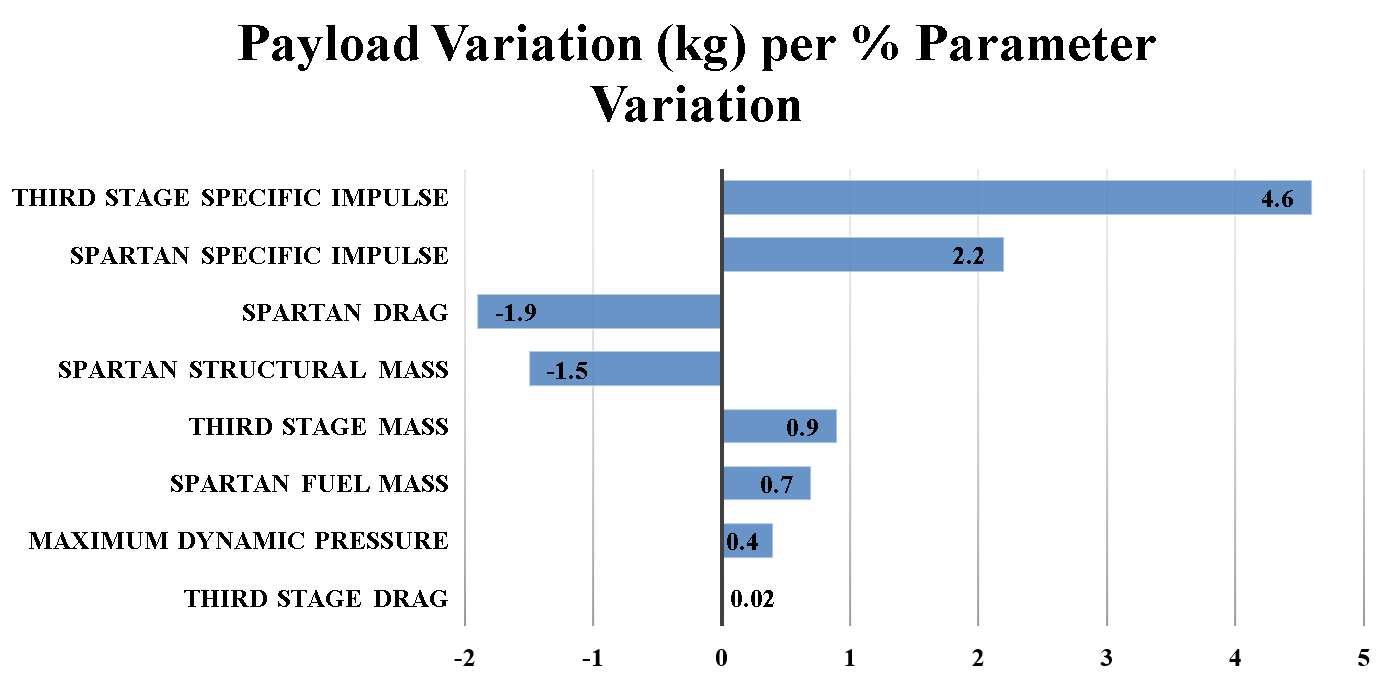
\includegraphics[width=0.99\linewidth]{figures/5_Ascent/BarChartRelativePayloadChange}
	\caption{The sensitivity of the key design parameters of the launch system.}
	\label{fig:BarChartRelativePayloadChange}
\end{figure}

\textcolor{red}{XXX I should be clear about why I am doing this - to inform future design decisions}

The preceding sections calculate the relative sensitivity of the launch system performance to a variety of design parameters. 
Comparing and contrasting the sensitivity of the launch system to each design parameter allows for the relative impact of each design parameter to be assessed. 
Figure \ref{fig:BarChartRelativePayloadChange} shows the change in payload mass per percentage point variation of each design parameter. 
This change per percentage variation indicates the magnitude by which the payload-to-orbit varies as each design parameter is varied by $\pm$1\% (signs are shown for positive parameter variations, with negative signs indicating a decrease in performance), and is measure of the sensitivity of the launch system to variations in each design parameter. 
However, a 1\% variation has a significantly different implication in the context of each individual design parameter, as certain parameters can be adjusted more easily. 
As such, the change per percentage is most useful when directly assessing each design parameter, and taking into account the associated effects on other, coupled design parameters. 

The influence of the maximum dynamic pressure of the scramjet accelerator on the performance of the launch system is low, particularly when compared to the influence of the closely linked scramjet accelerator mass parameter. These parameters are coupled directly, because the scramjet accelerator's thermal protective properties and structural strength define the maximum dynamic pressure. This means that the low variance in performance with maximum dynamic pressure may be offset by the variation in the mass of the scramjet accelerator, ie. a lower maximum dynamic pressure requires less structural and thermal protection system mass.
The relative sensitivities of the launch system to dynamic pressure (0.4$\frac{\Delta kg}{\Delta\%q_{max}}$), and scramjet accelerator mass (1.5$\frac{\Delta kg}{\Delta\%kg_{scramjet accelerator}}$), and their absolute magnitudes (50kPa and 4957kg respectively), allow the sensitivities of these coupled effects to be directly quantified. Comparing these sensitivities implies that so long as decreasing the dynamic pressure by 1kPa allows for a reduction in structural and TPS mass of greater than -26.5kg, then operating the scramjet accelerator at lower dynamic pressures may be preferable. 

The influence of the fuel mass of the scramjet accelerator on the performance of the launch system is also low, per percentage variation. However, the fuel mass is only a fraction of the total mass of the scramjet accelerator. This means that relatively small mass changes, by kg, in fuel mass are still significant. 
When the fuel mass of the scramjet accelerator is increased, the structural mass of the tanks will require a corresponding increase. 
Comparing the impact of the fuel mass and structural mass of the scramjet accelerator along with their relative magnitudes (1562kg of fuel mass and 4957kg of structural mass), the absolute impact of each is 0.044$\frac{\Delta kg_{payload}}{\Delta kg}$ and -0.030$\frac{\Delta kg_{payload}}{\Delta kg}$ respectively. This means that so long as fuel mass can be added to the scramjet accelerator with less than 1.47kg of structural mass incorporated for each 1kg of fuel mass, adding additional fuel mass will be beneficial. However, the fuel mass is constrained considerably by the available internal space within the scramjet accelerator, which is likely to be the main limiting factor.
If the size of the fuselage of the scramjet accelerator is increased, the aerodynamic performance of the scramjet accelerator will be altered proportionally. 
The sensitivity of the launch system to the drag of the scramjet accelerator, -1.9$\frac{\Delta kg}{\Delta\%C_{d}}$, means that so long as 1kg of fuel can be added to the scramjet accelerator with a drag increase of less than 0.024\%, then the maximum payload-to-orbit will increase. 


The payload-to-orbit is sensitive to the specific impulse of the C-REST engines, varying at a rate of 2.2$\frac{\Delta kg}{\Delta\%I_{SP}}$. Increasing the specific impulse of the scramjet engines is likely to require the addition of extra systems within the scramjet engines, adding weight to the scramjet accelerator, or a change in the shape of the scramjet engines, adding drag to the scramjet accelerator. 
The slightly lower sensitivity of the launch system to the scramjet accelerator mass (1.5$\frac{\Delta kg}{\Delta\%m_{scramjet accelerator}}$) compared to the sensitivity to the specific impulse, means that so long as increasing the $I_{SP}$ of the scramjet accelerator by 1\% causes a corresponding increase in the structural mass of the scramjet accelerator of less than 1.47\% (72.9kg), the performance of the launch system will improve. 
The sensitivity of the launch system to variation of the scramjet accelerator drag (1.9$\frac{\Delta kg}{\Delta\%C_d,{scramjet accelerator}}$) is similar in magnitude to the sensitivity to specific impulse. 
If a variation in the shape of the scramjet engines or forebody increases the $I_{SP}$ of the scramjet accelerator by 1\%, while increasing the drag of the scramjet accelerator by less than 1.16\%, then the efficiency of the launch system will be improved. 


 The specific impulse of the third stage rocket has the highest percentage payload variation effect on the launch system of any of the design parameters tested, at 4.6$\frac{\Delta kg}{\Delta\%I_{SP,3}}$. Increasing the specific impulse of the third stage is likely to involve modifications to the engine, increasing the pressure within the fuel tanks, or adding a turbopump to assist fuel flow, all of which involve increasing the mass of the third stage rocket. 
This additional mass is subtracted directly from the available payload mass of the system. This implies that so long as the specific impulse of the third stage can be increased by 1\% for less than 4.6kg additional engine and system mass, that the performance of the launch system will improve. 
However, increasing the specific impulse of the rocket engine is likely to add a large amount of cost to the third stage rocket, which is particularly detrimental, as the third stage is not reusable. This additional cost factor is likely to be the limiting factor on the specific impulse of the third stage rocket. 

 The aerodynamic performance of the third stage is shown to have only a very small impact on the performance of the launch system, with a drag sensitivity of only 0.02$\frac{\Delta kg}{\Delta\%C_{d,3}}$. This means that for any third stage shape variations, the aerodynamic sensitivity is small.
However, variations in the size of the third stage rocket are likely to require modifications in the size of the scramjet accelerator's fuselage. The sensitivity of the scramjet accelerator to drag, 1.9$\frac{\Delta kg}{\Delta\%C_d,{scramjet accelerator}}$, means that if the third stage can be enlarged so that the third stage mass increases by 1kg, with a corresponding enlargement of the fuselage of the scramjet accelerator so that the increase in scramjet accelerator drag is less than 0.014\%, the maximum payload-to-orbit will increase. 








\section{Summary}


In this chapter, LODESTAR was used to design the trajectory of the SPARTAN rocket-scramjet-rocket multi-stage launch system. 
A trajectory was simulated in which the scramjet accelerator stage flies at a constant dynamic pressure, producing \PayloadToOrbitConstqNoReturn kg of payload-to-orbit. This trajectory served to verify LODESTAR and the simulation of  the launch system, as well as providing a baseline trajectory for comparison. 
A trajectory optimised for maximum payload-to-orbit was then calculated, which increased the payload mass to sun synchronous orbit to \PayloadToOrbitStandardNoReturn kg (an increase of 19.5\%) compared to the constant dynamic pressure trajectory.
  The optimal flight path indicates that the optimal scramjet flight path for a system transitioning between separate airbreathing and rocket-powered stages involves the scramjet accelerator flying at less than its maximum dynamic pressure at three separate points along the trajectory. 
  Initially, the first-second stage separation occurs at a higher trajectory angle than in the constant dynamic pressure trajectory, causing the scramjet accelerator to fly at lower dynamic pressure, and trading off the exergy efficiency of the scramjet accelerator for an increase in the exergy efficiency and fuel mass of the first stage, for an overall performance gain. 
  The optimal flight path then exhibits an altitude raising manoeuvre in the middle of the trajectory, which improves the exergy efficiency of the scramjet accelerator by a very minor +0.003\%$\eta$ (+0.03\%). 
  Finally, the scramjet accelerator executes a pull-up manoeuvre before the second-third stage separation. This optimal pull-up manoeuvre trades off velocity (a decrease of 116.2m/s) for altitude (an increase of 9.48km) and improved flight path angle (an increase of 10.45$^\circ$). This pull-up manoeuvre, along with the higher first-second stage separation, decreases the exergy efficiency of the scramjet accelerator by -0.508\%$\eta$ (-9.7\%) when compared to the constant dynamic pressure case. 
  However, these conditions improve the exergy efficiency of the third stage rocket significantly, by +3.286\%$\eta$, an increase of +21.3\% over the third stage released from a constant dynamic pressure trajectory. 
 The pull up manoeuvre in the payload-to-orbit optimised trajectory also reduces the maximum dynamic pressure experienced by the third stage to 10.8kPa, a decrease of 43.4kPa compared to a trajectory with minimum pull-up, which allows future design benefits due to heat shield and structural mass reduction.  

A sensitivity study was conducted, to determine the relative effects of key vehicle design parameters on the optimised trajectory. 
The maximum dynamic pressure, specific impulse, aerodynamic performance, structural mass, and fuel mass of the scramjet accelerator were modified, along with the specific impulse, mass and aerodynamic performance of the third stage, and the magnitudes of their payload-to-orbit sensitivities compared. 
It was observed that the efficiency trade-off between the first stage and the scramjet accelerator depends primarily on the pitching ability of the first stage, so that when the first stage is capable of pitching more rapidly, the trade-off shifts in favour of the scramjet accelerator. 
The specific impulse of the third stage rocket was found to produce the most overall effect on the payload-to-orbit, increasing the payload by +45.9kg (+24.26\%) at 105\% $I_{sp}$, and decreasing the payload by -45.9kg (-24.26\%) at 95\% $I_{sp}$. However, increasing the specific impulse of the third stage rocket is likely to come at a high cost premium, which may be undesirable as the third stage is non-reusable. 
The most easily variable design factor, the maximum dynamic pressure of the scramjet accelerator, was found to have a relatively small effect on the payload-to-orbit performance of the launch system, varying the payload-to-orbit by only +24.2kg (+12.8\%) at 60kPa and -20.5kg (-10.8\%) at 40kPa. The negative effect on the payload-to-orbit when flying at 40kPa is likely to be offset by the lower TPS and structural mass required by lower dynamic pressure flight. It was determined that if the TPS and structural mass decrease is greater than -26.5kg for every 1kPa reduction in the maximum dynamic pressure, then flying at lower dynamic pressure is potentially preferable. 







